\documentclass[12pt]{article}  

\usepackage[boxruled,lined]{algorithm2e}
%% \usepackage{booktabs}
\usepackage{amsmath} 
\usepackage{amsthm} 
\usepackage{amsfonts} 
\usepackage{enumitem}
\usepackage{graphicx}
\usepackage[T1]{fontenc}
\usepackage{xparse} 
\usepackage{bm}
\usepackage{bbm} 
\usepackage{color,soul} 
\usepackage{framed}
\usepackage[margin=0.5in]{geometry}
\usepackage{listings}
\usepackage{hyperref}
\usepackage{mathtools}
\usepackage{multicol}
\usepackage[dvipsnames]{xcolor}
\usepackage{tikz}
\usepackage[normalem]{ulem}
\usepackage{pgfplots}  
\usepackage{pifont}
\usetikzlibrary{positioning}
\usetikzlibrary{calc}
\usetikzlibrary{fit}
\usetikzlibrary{shapes}
\usetikzlibrary{patterns}
\usetikzlibrary{decorations.pathreplacing}
\newcommand\STAR{{\tikz{\node[draw,star,star point height=.7em,minimum size=1em,scale=0.35]{};} }}
\newcommand{\Plus}{\mathord{\begin{tikzpicture}[baseline=0ex, line width=1, scale=0.13]
\draw (1,0) -- (1,2); \draw (0,1) -- (2,1); \end{tikzpicture}}}

\newtheorem{theorem}{Theorem}[section]
\newtheorem{lemma}[theorem]{Lemma}
\newtheorem{proposition}[theorem]{Proposition}
\newtheorem{corollary}[theorem]{Corollary}
\DeclarePairedDelimiter{\ceil}{\lceil}{\rceil}
\DeclarePairedDelimiter{\floor}{\lfloor}{\rfloor}
\DeclareMathOperator*{\argmin}{arg\,min}
\DeclareMathOperator*{\argmax}{arg\,max}
\newcommand{\D}{\mathrm{d}}
\SetKwInput{KwInput}{Input}
\SetKwInput{KwOutput}{Output}

\newcommand{\xdownarrow}[1]{%
  {\left\downarrow\vbox to #1{}\right.\kern-\nulldelimiterspace}
}

\newcommand{\xuparrow}[1]{%
  {\left\uparrow\vbox to #1{}\right.\kern-\nulldelimiterspace}
}

\begin{document}
\renewcommand{\d}[1]{\ensuremath{\operatorname{d}\!{#1}}}

\tableofcontents
\newpage
\section{Course Introduction}\vspace{.1pt} \hrule height 2pt \smallskip \renewcommand{\arraystretch}{1}
``The essence of reinforcement learning is memoized (context-sensitive) search'' -Barto and Sutton.
\vspace{-10pt}
\subsection{Motivating Reinforcement Learning}
Suppose you want to program a robot to collect cans that are laying around a messy lab. To do this naively, we'd first need to build a computer vision system that recognizes cans, obstacles, and people. Then, we'd need to construct a map of the environment and figure out how we can instruct the robot to learn \emph{where} it is in the map, i.e. the robot will need to localize itself. There's additional requirements as well, but let's consider an alternative. What if we were to use \emph{reinforcement learning}? In this example, the reward can be the number of cans the robot collects, and the agent could simply learn to collect as many cans as possible through trial and error. In principle, it wouldn't even need a map of the lab. In the event that a new type or color of can starts appearing in the lab, a reinforcement learning system would still learn to pick these up, whereas a pre-learned perception system would fail in this scenario. In order to make reinforcement learning work, we'll need (i) a good \emph{function approximation} if we want to learn from an on-board camera, as well as (ii) \emph{planning} so that the agent can revisit parts of the lab it hasn't been to in a while to check for new cans. The \emph{reward function} can simply be the total count of the number of cans collected at the \emph{end} of each day; this requires a TD-based algorithm to handle the delayed feedback.

\paragraph{Course Introduction} The promise of reinforcement learning is that an agent can figure out how the world works simply by trying things and seeing what happens. What's the difference between supervised learning, reinforcement learning, and unsupervised learning?
\begin{itemize}
\item In \emph{supervised learning}, we assume the learner has access to labeled   examples giving the correct answer.
\item In \emph{reinforcement learning}, the reward gives the agent an idea of how good or bad its recent actions were. While supervised learning is kind of like having a teacher that tells you what the correct \emph{answer} is, reinforcement learning is kind of like having someone tell you what good \emph{behavior} is, but they can't tell you exactly how to do it.
\item In \emph{unsupervised learning}, we try to extract the underlying structure of the data, i.e. data representation. Note that it's possible to use unsupervised learning to construct representations that make a supervised or RL system more performant.
\end{itemize}

\paragraph{Online Learning}
In RL, we focus on the problem of learning while interacting with an ever changing world. We do not expect our agents to compute a good behavior and then execute that behavior in an open-loop fashion. Instead, we expect our agents to sometimes make mistakes and refine their understanding as they go. The world is not a static place: we get injured, the weather changes, and we encounter new situations in which our goals change.  An agent that immediately integrates its most recent experience should do well especially compared with ones that attempt to simply perfectly memorize how the world works.
The idea of learning \emph{online} is an extremely powerful if not defining feature of RL. Even the way that this course introduces concepts tries to reflect this fact. For example, bandits and exploration will be covered before we derive inspiration from supervised learning. Getting comfortable learning \emph{online} requires a new perspective. Today, RL is evolving at what feels like breakneck pace: search companies, online retailers, and hardware manufacturers are exploring RL solutions for their day to day operations. There are convincing arguments to be made that such systems can be more efficient, save money, and keep humans out of risky situations. As the field evolves, it's important to focus on the fundamentals. E.g. DQN combines Q-learning, neural networks, and experienced replay. This course covers the fundamentals used in modern RL systems. By the end of the course, you'll implement a neural network learning system to solve an infinite state control task. We'll start with the multi-armed bandit problem: this introduces us to estimating values, incremental learning, exploration, non-stationarity, and parameter tuning.

\section{Multi-armed Bandits}
What distinguishes RL from other types of learning is that it uses training information that \emph{evaluates} the actions rather than \emph{instructs} by giving correct actions. Because we do not know what the \emph{correct} actions are, this creates the need for active exploration to search for good behavior.
\begin{itemize}
\item Purely evaluative feedback indicates how good the action was, but not   whether it was the best or the worst action possible.
\item Purely instructive feedback indicates the correct action to take, independently of the action actually taken.
\end{itemize}
To emphasize: evaluative feedback depends \emph{entirely} on the action taken, whereas instructive feedback is \emph{independent} of the action taken.
To start, we study the evaluative aspect of reinforcement learning in a simplified setting: one that does not involve learning to act in more than one situation. This is known as a \emph{non-associative} setting. We can then take one-step closer to the full RL problem by discussing what happens when the bandit problem becomes associative, i.e. when actions are taken in more than one situation.

\subsection{A $k$-armed Bandit Problem}
SUppose you are faced repeatedly with a choice among $k$ different options, or actions. After each choice you receive a numerical reward chosen from a \emph{stationary} probability distribution that depends on the action you selected. The objective is to maximize the expected total reward over some time-period e.g. $1,000$ action selections or \emph{time-steps}. Through repeated actions, we aim to maximize reward by concentrating actions on the best levers.

\paragraph{The expected reward of an action} In the $k$-armed bandit problem, each of the $k$ actions has an expected reward given that the action is selected; we refer to this quantity as the \emph{value} of an action. Denote the action selected at time step $t$ as $A_t$, and the corresponding reward as $R_t$. The value of an arbitrary action $a$, denoted by $q_*(a)$, is the expected reward given that $a$ is selected:
\[
  q_*(a) = \mathbb E \left[ R_t | A_t = a \right] = \sum_{r} \Pr(r|a) r
\]
If we knew the value of each action, the solution to the $k$-armed bandit problem is trivial: simply always select the action with highest value. But, we don't know the action values with certainy, instead we only have estimates: denote by $Q_t(a)$ the estimated value of action $a$ at time step $t$. We hope that $Q_t(a) \approx q_*(a)$.

\paragraph{Greedy actions} Suppose we maintain estimates of the action values. At any arbitrary time step, there is at least one action whose estimated value is greatest: these are called our \emph{greedy} actions. Selecting one of these is akin to \emph{exploiting} our current knowledge of the values of the actions. If we instead select a non-greedy action, then it is said we are \emph{exploring}, because this enables us to improve our estimate of the non-greedy action's value. Although exploitation is the obvious thing to do in a one-shot game, exploration may produce a greater total reward in the long run. Since it's not possible to both explore and to exploit with any single action selection, we often refer to a ``conflict'' between these strategies.

\paragraph{Balancing exploit-explore} In any specific case, whether it is better to explore or exploit depends in a complex way on the precise values of the estimates, their respective uncertainties, and the number of remaining time steps. There are sophisticated methods for balancing exploit-explore for particular formulations of the $k$-armed bandit and related problems, but most of these methods make strong assumptions about stationarity and prior knowledge that is often violated in practice. In this course, we focus not on an optimal balance between exploration and exploitation, but instead we worry about simply balancing them at all.

\subsection{Action-value Methods}
Let's consider methods for estimating the values of actions and for using these estimates to make subsequent action selection decisions; we collectively call these \emph{action-value} methods. We defined the true value of a reward as the mean reward when that action is selected, so it is natural to estimate this by averaging rewards actually received:
\begin{equation}
  \label{eq: sampleaveragemethodforactionvalue}
  Q_t(a) \coloneqq \frac{\textrm{sum of rewards when } a \textrm{ taken prior to } t}{\textrm{number of times } a \textrm{ taken prior to } t} = \frac{\sum_{i=1}^{t-1} R_i \cdot \mathbbm 1_{A_i = a}}{\sum_{i=1}^{t-1} \mathbbm 1_{A_i = a}}.
\end{equation}
Note that if the denominator is zero, we may instead define $Q_t(a)$ as some default value e.g. zero. Note that as the denominator tends to infinity, by the weak law of large numbers, $Q_t(a) \overset{p}{\longrightarrow} q_*(a)$, i.e. the sample mean converges in probability to the population mean. Equation
\ref{eq: sampleaveragemethodforactionvalue} defines a \emph{sample-average} method for estimate action values.

\paragraph{An action-selection rule} The simplest action-select rule is to chose among the set of actions with the highest estimated value. If there is more than one, we may select among them in an arbitrary way.
\[
A_t \coloneqq \argmax_a Q_t(a).
\]
Greedy action selection exploits our current knowledge to maximize immediate reward, and doesn't spend any time sampling seemingly inferior actions to see if they indeed may be better.

\paragraph{$\epsilon$-greedy Methods}
One alternative is to behave greedily most of the time, but every once in a while, say with probability $\epsilon$, to select randomly from among all the actions with equal probability, independently of the action-value estimates. This forms a class of $\epsilon$-greedy methods. An obvious advantage here is that in the limit as the number of steps increases, all actions will be sampled an infinite number of times,\footnote{To see this, realize that with an $\epsilon$-greedy method each action has probability at least $\epsilon > 0$ of being chosen at each time-step. For an arbitrary action $a$, the expected number of times we sample the action is given by $\sum_{t=1}^{\infty} \underbrace{\Pr(A_i = a)}_{\geq \epsilon}$ which diverges to $\infty$.} and this ensures that $Q_t(a) \overset{p}{\longrightarrow} q_*(a)$ for each action. Whence, the probability of selecting the optimal action converges to greater than $1-\epsilon$, i.e. to near certainty.\footnote{The reason for this last statement is quite obvious. Our strategy is to choose $A_t = \argmax_a Q_t(a)$ with probability $1-\epsilon$ and to sample among all possible actions with probability $\epsilon$, i.e. we choose $A_t$ with probability $1-\epsilon + \frac{\epsilon}{|\mathcal A|} > 1 - \epsilon$. By weak law of large numbers, in the limit we will have estimated each value precisely and so we have estimated the ordering of $Q_t(a)$ over all possible $a$, and so we are indeed selecting the optimal action with probability strictly greater than $1-\epsilon$.}

\subsection{The 10-armed Testbed} We propose a testbest on which to assess the relative effectiveness of the greedy and $\epsilon$-greedy action-value methods. Here, our $k$-armed bandit problem is for $k=10$. We replicate across $B$ bandit problems (e.g. $2,000$): for each bandit problem, the action values $q_*(a)$ are selected from a standard normal distribution; then, the reward for each action
is drawn from a normal distribution with unit variance and mean $q_*(a)$. For any learning method, we can measure its performance and behavior as it improves with experience for e.g. 1,000 time steps when applied to one instance of the bandit problem. Repeating for $B$ runs, each with a different bandit problem, we can obtain a measure of the learning algorithms average behavior.

\paragraph{Advantages of $\epsilon$-greedy methods} It depends on the task. If we have noisy rewards (i.e. they are drawn from a distribution with high variance), then it will take \emph{more} exploration to find the optimal action, and so we would expect the $\epsilon$-greedy method to fare better relative to the greedy method. If the reward variances are zero, then the greedy method would know the true value of each action aftery trying it once; in this case the greedy algorithm can quickly find the optimal action and then never explore. However, suppose we relax the problem a bit: if the bandit task is non-stationary, i.e. the true values of the actions evolve over time, then exploration is \emph{required} even in the deterministic case to ensure that one of the non-greedy actions has not changed to become better than the greedy one.

\subsection{Incremental Implementation} The action-value methods discussed so far all estimate action values as sample averages of observed rewards. How can we compute these efficiently? In particular, we want a running average that gets updated with constant memory and constant work required per update. To simplify notation let us concentrate on a single action. Let $R_i$ denote the reward received after the $i$th selection \emph{of this action}, and let $Q_n$ denote the estimate of its action value after it has been selected $n-1$ times, i.e.
\[
  Q_n \coloneqq \frac{R_1 + R_2 + \ldots + R_{n-1}}{n-1}.
\]
Note that a naive implementation would require more and more memory as more rewards are encountered. Instead, realize that given $Q_n$ and the $n$-th reward $R_n$, the new average of all $n$ rewards can be computed by
\begin{align}
  Q_{n+1} &= \frac{1}{n} \sum_{i=1}^n R_i &\textrm{definition of } Q_{n+1}\nonumber \\
          &= \frac{1}{n} \left( R_n + \sum_{i=1}^{n-1} R_i \right) &\textrm{breaking apart summation}\nonumber  \\
          &= \frac{1}{n} \left(R_n + \frac{n-1}{n-1} \sum_{i=1}^{n-1} R_i\right) &\substack{\textrm{multiplying by 1} \\ \textrm{to make an average appear}}\nonumber    \\
          &= \frac{1}{n} \left(R_n + \left(n-1\right) Q_n \right) &\textrm{By definition of } Q_n \nonumber  \\
          &= \frac{1}{n} \left(R_n + nQ_n - Q_n \right) &\textrm{factoring out terms}\nonumber  \\
  \label{eq: incrementalimplementation}
          &= Q_n + \frac{1}{n} \left[R_n - Q_n \right] &\textrm{algebraic simplification}
\end{align}
What's nice is that \ref{eq: incrementalimplementation} holds even for $n=1$, in which case we get that $Q_2 = R_1$ for arbitrary $Q_1$. Notice that we only have to store $Q_n$ and $n$, and the perform the work required by \ref{eq: incrementalimplementation} at each time step. What's interesting about this update rule is that it actually reoccurs frequently throughout this book:
\[
  \texttt{NewEstimate} \gets \texttt{OldEstimate} + \texttt{StepSize} \left[ \underbrace{\texttt{Target} - \texttt{OldEstimate}}_{\textrm{\emph{error}}} \right]
\]
The expression $\texttt{Target} - \texttt{OldEstimate}$ is an \emph{error} in our estimate which is reduced by taking a step towards the ``target'', which is presumed to indicate a desireable direction in which to move albeit may be subject to noise. In the case of our sample-average action-value method, the target is the $n$-th reward.
\paragraph{Step-size parameter} Note that there is a parameter \texttt{StepSize} that appears in \ref{eq: incrementalimplementation} which can depend upon the time step. In processing the $n$-th reward for action $a$, the sample-average action-value method uses the step size parameter $\frac{1}{n}$. In general, we denote the step size parameter by $\alpha_t(a)$.
\paragraph{A simple bandit algorithm} We now write out pseudo-code for a complete bandit algorithm using incremental updates for our sample-averages and an $\epsilon$-greedy action selection strategy.
\begin{algorithm}
  \For{$a = 1, \ldots, k$}{
    $Q(a) \gets 0$ \\
    $N(a) \gets 0$
  }
  \While{True}{
    $A \gets \begin{cases}\argmax_a Q(a) &\textrm{ with probability } 1-\epsilon \hspace{15pt} (*\textrm{breaking ties randomly}) \\ \textrm{random action} &\textrm{ with probability } \epsilon     \end{cases}$ \\
$R \gets \texttt{Bandit}(A)$ \\
$N(A) \gets N(A) + 1$ \\
$Q(A) \gets Q(A) + \frac{1}{N(A)} \left[R - Q(A) \right]$
}
\caption{A simple $\epsilon$-greedy $k$-armed bandit algorithm}
\end{algorithm}
Here, the function $\texttt{Bandit}(\cdot)$ accepts an action as argument and returns a corresponding reward.
\subsection{Tracking a Nonstationary Problem using Exponentially Weighted Moving Averages} The sample-average action-value methods described so far are only appropriate for stationary bandit problems, i.e. ones in which the reward probabilities don't change over time. In cases of non-stationarity, it makes sense to give more weight to recent rewards than to long-past rewards. One of the ways to accomplish this is by using a \emph{constant} step size parameter. For example we can change \ref{eq:   incrementalimplementation} to something like
\begin{equation}
  \label{eq: incrementalupdateweightedaverage}
  Q_{n+1} \coloneqq Q_n + \alpha \left[ R_n - Q_n \right]
\end{equation}
where the step size $\alpha \in (0, 1]$ is constant. Realize that this results in $Q_{n+1}$ being a weighted average of past rewards, given an initial estimate $Q_1$:
\begin{align}
  Q_{n+1} &= Q_n + \alpha \left[R_n - Q_n \right] &\textrm{by equation \ref{eq: incrementalupdateweightedaverage}}\nonumber \\
          &= \alpha R_n + \left(1-\alpha\right) Q_n &\textrm{re-arranging terms} \nonumber \\
          &= \alpha R_n + \left(1-\alpha\right) \left[\alpha R_{n-1} +             (1-\alpha)Q_{n-1}\right] &\substack{\textrm{substituting for } Q_n \\ \textrm{ based on pattern observed above}} \nonumber \\
          &= \alpha R_n + (1-\alpha)\alpha R_{n-1} + (1-\alpha)^2 Q_{n-1} &\textrm{distributing } (1-\alpha) \nonumber \\
          &= \alpha R_n + (1-\alpha)\alpha R_{n-1} + (1-\alpha)^2 \alpha R_{n-2}             + \ldots + (1-\alpha)^{n-1} \alpha R_1 + (1-\alpha)^n Q_1 &\substack{\textrm{iteratively plugging in} \\ \textrm{for } Q_i} \nonumber  \\
          &= \underbrace{(1-\alpha)^n Q_1}_{f(\textrm{initial value})} + \underbrace{\sum_{i=1}^{n} \alpha (1-\alpha)^{n-i} R_i}_{\textrm{weighted average of rewards}}. \label{eq: expoweightedaveragenonstationaryproblem}
\end{align}
Note that the sum of the weights is given by $(1-\alpha)^n + \sum_{i=1}^n \alpha (1-\alpha)^{n-i} = 1$. Note that crucially, the weight $\alpha(1-\alpha)^{n-i}$ given to the reward $R_i$ depends on how many rewards ago, $n-i$, that it was observed. Since $\alpha \in (0,1]$, the quantity $1-\alpha < 1$, thus the weight given to $R_i$ decreases as the number of intervening rewards increases. In fact, the weight decays exponentially according to the exponent on $1-\alpha$.\footnote{If $1-\alpha=0$, then all the weight goes to the very last   reward $R_n$, because of the convention that $0^0=1$.} Further, our initial value matters less and less the more data we obtain.

\paragraph{Varying Step-Size Parameter from step-to-step} Let $\alpha_n(a)$ denote the step-size parameter used to process the reward received after the $n$-th selection of action $a$. The choice of $\alpha_n(a) = \frac{1}{n}$ results in the sample-average action-value strategy, which is guaranteed to converge to the true action-values by the weak law of large numbers. But, convergence isn't guaranteed for all choices of the sequence $\{\alpha_n(a)\}$. To ensure convergence with probability 1, we require that
\begin{equation}
  \sum_{n=1}^{\infty} \alpha_n(a) = \infty \hspace{25pt} \textrm{ and } \hspace{25pt} \sum_{n=1}^{\infty} \alpha_n^2(a) < \infty.
\end{equation}
The first condition is required to guarantee that the steps are large enough to eventually overcome any initial conditions (i.e. that we revisit actions infinitely many times), and the second condition guarantees that eventually, the step sizes become small enough to assure convergence. Note that both conditions are met for the sample-average case of $\alpha_n(a) = \frac{1}{n}$, but \emph{not} for the case of the constant step size parameter $\alpha_n(a) = \alpha$. In the latter case, the second condition isn't met, indicating that the estimates may never completely converge but instead continue to vary in response to the most recently received rewards; this is actually \emph{desireable} in the nonstationary environment.

\subsection{Optimistic Initial Values} Our methods discussed thus far depend to some extent on initial action-value estimates $Q_1(a)$, i.e. we are \emph{biased} by our initial estimates. For sample-average methods, the bias dissappears once all actions have been selected at least once. But, for methods with constant $\alpha$, the bias is permanent albeit decreasing over time as given by equation \ref{eq: expoweightedaveragenonstationaryproblem}. Although this kind of bias can sometimes be helpful, the downside is that the initial estimates become a set of parameters that must be picked by the user, if only to set them all to zero. The upside is that they provide an easy way to encode prior knowledge about what levels of rewards can be expected.

\paragraph{Encouraging early exploration through large initial action values} Suppose that instead of setting initial action valus to zero in the 10-arm testbed, that we instead set them to $+5$. Note that based on our simulation we drew $q_*(a)$ from a standard normal, and so an initial estimate of $+5$ is wildly optimistic. What happens is that whichever action(s) are initially selected, the reward will always be less than the initial estimates and the algorithm will be encouraged to continue exploring all possibilities at least once. The system does a fair bit of exploration even if the greedy action-value strategy is employed! This technique can be particularly effective on stationary problems: initially the optimistic method performs worse than $\epsilon$-greedy because it explores more often, but eventually it performs \emph{better} because its exploration decreases with time. Note that the method is ill-suited to nonstationary problems since the drive for exploration is temporary. Note that in practice, it may not be obvious what an ``optimistic'' initial value is, since we may not know what is a maximal reward.

\subsubsection{Unbiased constant-step-size trick} Sample averages are not satisfactory because they do not perform well on nonstationary problems. Consider a step size of
\[
  \beta_n = \alpha / \bar{o}_n,
\]
to process the $n$-th reward for a particular action, where $\alpha > 0$ is a conventional constant step size, and $\bar{o}_n$ is a trace of one that starts at 0:
\begin{align*}
  \bar{o}_n &\coloneqq \bar{o}_{n-1} + \alpha(1-\bar{o}_{n-1}) &\textrm{for } n \geq 0, \hspace{10pt} \textrm{ with } \bar{0}_0 = 0.
\end{align*}
\subsection{Upper-confidence bound action selection}
\paragraph{Optimism in the face of uncertainty}
We require exploration since there is always uncertainty about the accuracy of our action-value estimates. Greedy actions have been defined as the set of actions which look best at present, but it's possible that other actions could be better. The $\epsilon$-greedy action selection method forces the non-greedy actions to be tried, but indiscriminately, with no preference for those that are near greedy or particularly uncertain. Wouldn't it be nice if we could select among the non-greedy actions according to their potential for actually being optimal, taking into account both how close their estimates are to being maximal and the uncertainties in those estimates? One effective method is upper-confidence bound action selection:
\[
  A_t \coloneqq \argmax_a \left[ \underbrace{Q_t(a)}_{\textrm{exploit}} + c \underbrace{\sqrt{\frac{\ln t}{N_t(a)}}}_{\textrm{explore}}\right]
  \]
  where $c>0$ controls the degree of exploration. If $N_t(a) = 0$ we consider $a$ to be a maximizing action. The fundamental idea is that the square root term is a measure of uncertainty or variance in the estimate of $a$'s value. The quantity being maximized over is an upper bound on the true value of action $a$, with $c$ determining the confidence level. Each time some $a$ is selected, its uncertainty is presumably reduced: $N_t(a)$ increments, and as it appears in the denominator, the uncertainty term decreases. On the other hand, each time an action other than $a$ is selected, $t$ increases, but $N_t(a)$ doesn't, and because $t$ appears in the numerator the uncertainty estimate increases. The use of the natural logarithm means that the increases get smaller over time, but they are unbounded; i.e. all actions will eventually be selected, but actions with lower value estimates, or those that have already been selected frequently, will be selected with decreasing frequency over time.

\subsection{Sequential Decision Making with Evaluative Feedback} In RL, the agent generates its own training data by interacting with the world. The agent must learn the consequences of their actions through trial and error, rather than being told what correct actions are. Let's focus on the evaluative asepect of RL; in particular we will formalize the problem of decision making under uncertainty using $k$-armed bandits, and we will use this as a foundation to discover fundamental RL concepts such as rewards, timesteps, and values.

\paragraph{Motivating Example: Medical Treatments} Imagine a medical trial where a doctor wants to measure the effectiveness of three different treatments. Whenver a patient comes into the office, the doctor prescribes a treatment at random. After a while, the doctor notices that one treatment seems to be working better than the others. The doctor is now faced with a decision: should he/she stick with the best-performing treatment, or continue with the randomized study? If the doctor only prescribes one treatment, they can no longer collect data on the other two, and what if its the case that one of the other treatments is actually better (it only happens to appear worse due to random chance)?

\paragraph{Making RL work in Real Life} You want to shift your priorities.

\begin{tabular}{l | r}
  Important to RL, but should be Less Important in Real Life & Important in Real                                                                Life \\
  \hline
  Temporal credit assignment & Generalization across observations \\
  Control environment & Environment controls \\
  Computational efficiency & Statistical efficiency \\
  State & Features \\
  Learning & Evaluation \\
  Last policy & Every policy
\end{tabular}

In RL, computational efficiency is paramount, since we are running simulations and we have as many observations as we can compute; but in real life we are often more focused on statistical efficiency since the number of observations are fixed.
As another example, we may have a 1 megapixel camera, but do we really need to capture all of that information as part of our state? Perhaps a higher representation suffices. Lastly, in RL we only care about the last policy since we're running our simulations for a very long time; but in the real world every observation involves some interaction with the world, so we want the performance to always be pretty good, i.e. we care about the entire trajectory of policies.

\paragraph{Contextual Bandits}
Suppose that there are several different $k$-armed bandit tasks, and that on each step you confront one of these chosen at random. The bandit task is changing randomly from step to step. This would appear to the agent as a single, non-stationary $k$-armed bandit task whose true action values change randomly from step to step. Unless the true action values change very slowly, the methods described so far won't work. But now imagine that when a bandit task is selected for you on each round, you are given a distinctive clue about its identity (but not the action values), e.g. you are facing an actual slot machine that changes color of its display as it changes the action values.\footnote{In contextual bandits, we observe some features  $x$. Perhaps its the geolocation of the user, the profile based on the way the  user has behaved in the past, maybe it's features of possible actions which are available as well.} Now, you can learn a policy associating each task, signaled by the color you see, with the best action to take when faced with that task. This is an example of an \emph{associative search} task, so called because it involves both trial-and-error learning to \emph{search} for the best actions as well as the \emph{association} of these actions with the situations in which they are best.
Associative search tasks are often called \emph{contextual bandits} in the literature.

\paragraph{Thompson Sampling} There is a family of Bayesian methods which assume an initial distribution over the action values and then update the distributionexactly after each step (assuming that the true action values are stationary). In general, the update computations are complex, but for conjugate priors they are straightforward. One possibility is to then select actions at each step according to their \emph{posterior} probability of being the best action. This method, sometimes called \emph{posterior sampling} or \emph{Thompson sampling}, often performs similarly to the best of the distribution-free methods we've gone over so far. In the Bayesian setting, it's conceivable to compute the \emph{optimal} balance between explore/exploit. For any possible action, one can compute the probability of each possible immediate reward and the resultant posterior distributions over action values. This \emph{evolving} distribution becomes the \emph{information state} of the problem. Given a horizen of $T$ time-steps, one can consider all possible actions, all possible resulting rewards, all possible next actions, all next rewards, and so on for $T$ time steps. Given the assumptions, the rewards and the probabilities of each possible chain of events can be determined, and one can simply pick the best. The problem is computationally intractable, however, as the tree of possibilities grows exponentially.

\section{Finite Markov Decision Processes}
Suppose we have a rabbit who prefers carrots over broccoli, each having reward $+10$ and $+3$ respectively. In the first time step, the rabbit can move \emph{right} to get a carrot or left to get broccoli: clearly it prefers to move right to get the highest reward. But at a later time step the situation is reversed, where the rabbit can now move \emph{left} to get a carrot or right to get broccoli. Clearly the rabbit should take the action of moving left. Or, consider another example where on the other side of the carrot is a predator: now the rabbit should prefer to take the broccoli since it'll have a better chance of survival in the long run (what looks good in the short-term isn't always what's best in the long-term). Note that the $k$-armed bandit does not account for the sequential decision making process as described here.

\paragraph{MDPs}
The problem involves evaluative feedback, as in the case of bandits, but additionally there is an associative aspect of choosing different actions in different situations.  MDPs are a classical formalization of sequential decision making, where actions influence not only immediate rewards but also subsequent situations, or states, and through those future rewards. In MDPs we estimate the value $q_*(s,a)$ of each action $a$ in each state $s$, or we estimate the value
$v_*(s)$ of each state given optimal action selections. In this new framework, the agent and environment interact with each other. At each time step, there is a set of possible states the agent can be in $S_t \in \mathcal S$, and there is correspondingly a (subset of) actions they make take $A_t \in \mathcal A(S_t)$.

\begin{figure}[h]
  \centering
  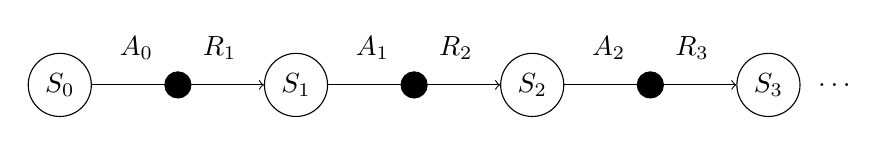
\begin{tikzpicture}
  \foreach \x in {0, 1, 2, 3} {
    \node[draw,circle] (s\x) at (\x*3, 0) {$S_{\x}$};
  }
  \foreach \x in {0, 1, 2} {
    \node[draw,circle,fill] (inter\x) at (\x*3+3/2, 0) {};
    \node[above left = 1mm of inter\x] {$A_\x$};
  }
  \node[above right = 1mm of inter0] {$R_{1}$};
  \node[above right = 1mm of inter1] {$R_{2}$};
  \node[above right = 1mm of inter2] {$R_{3}$};
  \draw[->] (s0) -- (s1);
  \draw[->] (s1) -- (s2);
  \draw[->] (s2) -- (s3);
  \node[right = 1mm of s3] {$\ldots$};
\end{tikzpicture}
\caption{\footnotesize Here we represent the sequential nature of an MDP. At each time step, the agent finds itself in a given state. It takes an action which results in some reward. The process then repeats itself (perhaps indefinitely).}
\end{figure}

\paragraph{Dynamics of an MDP} As in bandits, the outcomes of our action-state pairs are stochastic and so we may use the language of probability. When the agent takes an action in a state, there are many possible next states and rewards. The transition dynamics function $P$ formalizeds this notion. Given a state $s$ and action $a$, $p$ instructs us of the joint probability of the next state $s'$ and reward are, i.e. $\Pr(s', r | s, a)$. In this course, we assume the set of states, actions, and rewards are finite, although we will learn about algorithms that can handle infinite and uncountable sets. Since $p$ is a probability distribution, it must be non-negative and its sum over all possible next states and rewards must equal one. I.e. $p : \mathcal S \times \mathcal R \times \mathcal S \times \mathcal A \to [0,1]$, and
\[
  \sum_{s' \in \mathcal S} \sum_{r \in \mathcal R} \Pr(s', r | s, a) = 1, \hspace{15pt} \forall s \in \mathcal S \hspace{5pt} a \in \mathcal A(s)
\]
Note that the future state and reward depend only on the current state and action. In writing our probability in this way, we have defined a Markov process, and it intuitively means that the present state is sufficient and that remembering earlier states or trajectories would not improve predictions about the future.

\subsection{Returns and Episodes} An agents goal is to maximize the cumulative reward it receives in the long run. If the sequence of rewards received after time step $t$ is denoted by $R_{t+1}, R_{t+2}, \ldots$, each a random variable, then what precise aspect of this sequence do we wish to maximize? In general, we seek to maximize \emph{expected} return, where the return at time step $t$, denoted by $G_t$,
is some specific function of the reward sequence. In the simplest case the return is the sum of rewards:
\begin{equation}
  \label{eq: sumofrewards}
  G_t \coloneqq R_{t+1} + R_{t+2} + \ldots + R_T
\end{equation}
where $T$ is a final time step. This approach really only makes sense in applications where there is a notion of a final time step, i.e. when the agent-environment interaction naturally breaks into subsequences, which we call \emph{episodes}. Example episodes are plays of a game, trips through a maze, or any sort of repeated interaction; episodes end in a special \emph{terminal state}, followed by a reset to a standart starting state or to a sample from a standard distribution of starting states. No matter how the last episode finished, e.g. win or lose, the next episode begins independently of how the previous one ended.  Tasks with episodes of this kind are called \emph{episodic} tasks; in such tasks we sometimes distinguish the set of all non-terminal states $\mathcal S$ from the set of all states plus the terminal state, denoted by $\mathcal S^+$. Note that the time of termination $T$ is a random variable that varies from episode to episode.

\paragraph{Effect of adding a constant to all rewards in an episodic task}
Note that if we add a constant to all rewards in an episodic task, then this may change the set of optimal policies. To see this, realize that adding a constant to the reward signal can make \emph{longer} episodes more or less advantageous, depending on whether the constant is positive or negative.

\paragraph{Examples of episodic tasks}
One example of an episodic task is a game of chess; it always ends in either a checkmate, draw, or resignation, and a single game constitutes an episode. Each game starts from the same start state with all pieces reset. The state is given by the position of all the pieces on the board, and the actions are all the legal moves. We could define the reward as $+1$ for winning and zero for all other moves. Another example is the case of an agent learning to play a video game, in which the player gets a point for collecting treasure blocks and dies when they touch an enemy. This game is clearly an episodic MDP: the agent tries to get a high score, collecting as many points as possible before the game ends. The state is an array of pixel values corresponding to the current screen. There are four actions: up, left, down, right. The agent gets a reward of $+1$ every time they collect a treasure block. An episode ends when the agent touches one of the enemies. Regardless of how the episode ends, the next episode begins in the same way, with the agent at the center of the screen with no enemies present.

\subsection{Continuing Tasks} In many cases, the agent-environment interaction doesn't break naturally into identifiable episodes, but instead goes on continually without limit; e.g. a process-control task, or an application to a robot with a long life span. We call these \emph{continuing tasks}. The definition of return as in equation \ref{eq: sumofrewards} is problematic because the final time step would be $T =\infty$, and the return (which we are trying to maximize) could itself be divergent. For example, suppose an agent receives a reward of $+1$ at each time step. To address this issue, we use discounting.

\paragraph{Effect of adding a constant to all rewards in continuing tasks on the set of optimal policies}
Note that if we add a constant to all rewards in a continuing task, then the agent will accumulate the same amount of extra reward independent of its behavior, and so the set of optimal policies will not change.

\paragraph{Discounting Returns} In this approach, the agent tries to select actions so that the sum of the discounted rewards it receives over the future is maximized. I.e. it selects $A_t$ to maximize the expected \emph{discounted   return}:
\begin{equation}
  \label{eq: discounted return}
  G_t \coloneqq R_{t+1} + \gamma R_{t+2} + \gamma^2 R_{t+3} + \ldots = \sum_{k=0}^{\infty} \gamma^k R_{t+k+1},
\end{equation}
where $\gamma \in [0,1]$ is called the \emph{discount rate}. This rate determines the present value of future rewards: a reward received $k$ time steps in the future is worth only $\gamma^{k-1}$ times what it would be worth if it were received immediately.\footnote{Intuitively, this makes sense: a dollar today is worth more to you than a dollar in a year.} Note that if $\gamma < 1$, then our discounted reward in equation \ref{eq: discounted return} is convergent so long as the reward sequence $\{R_k\}$ is bounded. If $\gamma = 0$, the agent is myopic and only focuses on maximizing immediate reward: its objective becomes choose $A_t$ so as to maximize only $R_{t+1}$. If it happened to be the case that the agent's actions influenced \emph{only} the immediate reward, not future rewards as well, then a myopic agent could maximize \ref{eq: discounted return} by separately maximizing each immediate reward.  But, in general acting to maximize the immediate reward can reduce access to future rewards so that the return is reduced. On the other hand, as $\gamma \leadsto 1$, the return objective takes future rewards into account more strongly and the agent becomes farsighted. Note that
\begin{align}
  G_t &\coloneqq R_{t+1} + \gamma R_{t+2} + \gamma^2 R_{t+3} + \gamma^3 R_{t+4}         + \ldots \nonumber \\
      &= R_{t+1} + \gamma \left(R_{t+2} + \gamma R_{t+3} + \gamma^2 R_{t+4} +                 \ldots \right) \nonumber \\
  \label{eq: recursivereturnformulation}
      &= R_{t+1} + \gamma G_{t+1}.
\end{align}
This works for all time steps $t<T$, even if termination occurs at $t+1$, so long as we define $G_T = 0$. Even though our return \ref{eq: discounted return}
is an infinite sequence, it is finite if the reward is non-zero and constant and if $\gamma < 1$. E.g. if the reward is a constant $+1$ then $G_t = \sum_{k=0}^{\infty} \gamma^k = \frac{1}{1-\gamma}$.

\paragraph{Proof of convergence} Let's examine why it's the case that $G_t < \infty$ if $\gamma < 1$. Assume that $R_{\textrm{max}}$ is the maximum reward our agent can achieve at any time step. We can upper bound the return $G_t$ by replacing every reward with $R_{\textrm{max}}$, and since it's just a constant we can then pull it out of the sum. We're left with a (scaled) geometric series which converges since $\gamma < 1$:
\begin{align*}
  G_t = \sum_{k=0}^{\infty} \gamma^k R_{t+k+1} \leq \sum_{k=0}^\infty \gamma^k R_{\textrm{max}} = R_{\textrm{max}} \sum_{k=0}^\infty \gamma^k = R_{\textrm{max}} \frac{1}{1-\gamma}.
\end{align*}

\paragraph{Examples of Continuing tasks} Consider a smart thermostat which regulates the temperature of a building. This can be formulated as a continuing task since the thermostat never stops interacting with the environment. The state could be the current temperature, along with details of the situation like the time of day and the number of people in the building. There are just two actions: turn on the heater or turn it off. The reward can be $-1$ every time someone has to manually adjust the temperature and zero otherwise. To avoid negative reward, the thermostat would learn to anticipate the user's preferences. Another example is an agent scheduling jobs on a set of servers. Suppose we have three servers used  by reinforcement learning researchers to run experiments. Researchers submit jobs with different priorities to a single queue. The state is a number of free servers, and the priority to the job at the top of the queue. The actions are to reject or accept the job at the top of the queue if a server is free. Accepting the job runs it and yields a reward equal to the job's priority. Rejecting a job yields a negative reward proportional to the priority, and sends the job to the back of the queue. Note that the agent must be careful about scheduling low-priority jobs, since this could prevent high priority jobs from being scheduled later. The servers become available as they finish their jobs. The researchers continually add jobs to the queue, and the agent accepts or rejects them; the process never stops!  It's well-described as a continuing task.

\subsection{Examples of MDPs}
The MDP framework can be used to formalize a wide variety of sequential decision-making problems.
Consider our recycling robot which collects empty soda cans in an office environment: it can detect soda cans, pick them up using a gripper, and then drop them off in a recycling bin. The robot runs on a rechargeable battery, and its objective is to collect as many cans as possible. To formulate this problem as an MDP, we start with the states, actions, and rewards. Suppose the sensors can only distinguish between two levels of battery charge: \texttt{high} and \texttt{low}, and these represent the robot's state. In each state, the robot has three choices: it can search for cans for a fixed amount of time, it can remain stationary and wait for someone to bring it a can, or it can go to the charging station to recharge its battery. We'll only allow charging from low battery state since charging otherwise is pointless. Now, let us consider transition dynamics as per figure \ref{fig: mdprobotrecycler}.

\begin{figure}[h]
  \centering
  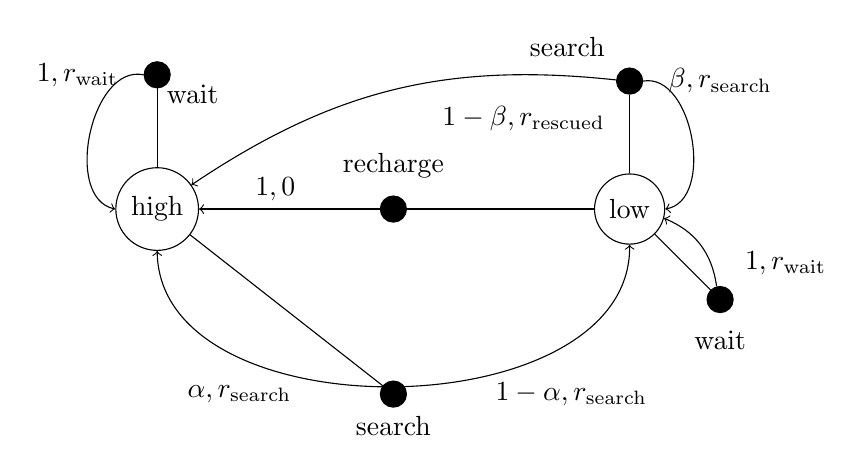
\begin{tikzpicture}
    \node[draw,circle] (hi) at (0,0) {high};
    \node[draw,circle] (lo) at (6,0) {low};
    \path[<->] (hi) edge[bend right=90] (lo);
    \draw[-] (hi) -- (3, -2.35) node[draw,circle,fill] (hi_search) {};
    \node at (3,-2.75) {search};
    \node[left=10mm of hi_search] (hilabel) {$\alpha, r_{\textrm{search}}$};
    \node[right=10mm of hi_search] (lolabel) {$1-\alpha, r_{\textrm{search}}$};
    \node[above=of hi, draw,circle, fill] (wait_hi) {};
    \draw[-] (hi) -- (wait_hi) node[below right] {wait};
    \path[->] (wait_hi) edge[bend right = 90] (hi) node[left = 2mm of wait_hi]     {$1,r_{\textrm{wait}}$};
\node[above=of lo, draw,circle, fill] (search_lo) {};
\draw[-] (lo) -- (search_lo);
\node[above left = 1mm of search_lo] {search};
    \draw[->] (search_lo) edge[bend left = 90] (lo) node[right = 2mm of     search_lo] {$\beta, r_{\textrm{search}}$};
    \draw[->] (search_lo) edge[bend right = 20] (hi) node[below left = 1mm of         search_lo] {$1-\beta, r_{\textrm{rescued}}$};
\draw[->] (lo) -- (hi);
\node[draw,circle,fill] (recharge) at (3,0) {};
\node[above=1mm of recharge] {recharge};
\node at (1.5, 0.25) {$1,0$};
\node[below right=1cm of lo,draw,circle,fill] (lo_wait) {};
\node[below=1mm of lo_wait] {wait};
\draw[-] (lo) -- (lo_wait);
\path[->] (lo_wait) edge[bend right = 30] (lo);
\node[above right = 1mm of lo_wait] {$1,r_{\textrm{wait}}$};
  \end{tikzpicture}
  \caption{\footnotesize The \emph{state} of the robot's battery is indicated by open nodes in the graph, demarcated by ``high'' and ``low''. Actions are denoted by coloured nodes, and an edge between a state-action pair indicates that it is possible to execute said action from the corresponding state. After taking an action we observe a reward, and also a state change with some specified probability; for each transition we indicate the probability of transition and also the reward as a comma separated tuple alongside the corresponding edge. Hypothetical reward values: $r_{\textrm{wait}} = 1$, $r_{\textrm{search}} = 10$, $r_{\textrm{rescued}} = -20$. In our problem, $\alpha, \beta \in [0,1]$ describe transition probabilities when searching from a high or low battery state respectively.}
\label{fig: mdprobotrecycler}
\end{figure}

\paragraph{Extensibility of MDPs}
The MDP framework is highly extensible, and can be used in many applications. States can be low-level sensory readings, for example, in the pixel values of the video frame. They could also be high-level such as object descriptions. Similarly, actions could be low level, such as the wheel speed of the robot, or they could be high level, such as ``go to the charging station''. Time steps can be very small or very large, for example they can be one millisecond or one month; they can either be fixed intervals of time or successive stages of decision making.

\paragraph{Pick-and-place task} Suppose we want to use RL to control a robot arm in which the goal of the robot is to pick up objects and place them in a particular location. There are many ways we could formalize this task, but here's one. The \emph{state} could be the readings of the joint-angles and velocities. The \emph{actions} could be the voltages applied to each motor. The \emph{reward} could be $+100$ for successfully placing each object. But, we also want the robot to use as little energy as possible, so let's include a small negative reward corresponding to energy used, e.g. $-1$ for each unit of energy consumed.

\paragraph{Reward functions} Consider a robot learning to walk. The reward could be proportional to the forward motion. Lurching forward clearly maximizes immediate reward, however this action causes the robot to fall over. If the robot instead maximizes total forward motion instead, it would walk quickly but carefully. To teach an agent how to escape from a maze, the reward might be $-1$ for each time step that passes prior to escape, encouraging the agent to escape as quickly as possible. For an agent learning to play checkers or chess, the natural rewards might be $+1$ for winning, $-1$ for losing, and $0$ for drawing and for all non-terminal positions. In a stock market, we can use monetary rewards to optimize: since buying actions cost dollars, selling actions generate dollars, and the trade-offs are quite simple.
\begin{itemize}
\item \textbf{Goal rewarding encoding:} define a state where the goal is achieved as   having $+1$ reward and all other states yield zero reward.
\item \textbf{Action penalty representation:} penalize the agent with a $-1$ each step in which the goal has not been achieved.
\end{itemize}
Both these formulations achieve optimal behavior by reaching the goal, eventually. But, what the agent does along the way is subtly different. Goal rewarding encoding doesn't really encourage the agent to get to the goal with any sense of urgency, and action penalty representation runs into serious problems if there is some small probability of getting stuck and never reaching the goal. Both schemes can lead to big problems for goals with \emph{really} long horizons, e.g. consider encouraging an agent to win a Nobel Prize. Just giving an agent a reward for attaining the ultimate goal is quite a tough sell. Some intermediate rewards like doing well on a science test or earning tenure could make a difference in orienting the agent in the right direction.

\subsection{The reward hypothesis}
The hypothesis states ``that all of what we mean by goals and purposes can be well thought of as the maximization of the expected value of the cumulative sum of a received scalar signal (called reward)''.
There are three ways to think about creating intelligent behavior.
\begin{itemize}
\item Give a man a fish. If we want a machine to be smart, we program it with the behavior we want it to have. But, as new problems arise, the machine won't be able to adapt to new circumstances. It requires us to always be there providing new programs.
\item Teach a man to fish. This is supervised learning: provide training examples and the machine writes its own program to match those examples. It learns, so long as we have a way to provide training examples, our machine will be able to write its own programs, and that's progress. But situations change.
\item Give a man a taste for fish. This is reinforcement learning. The idea is that we don't have to specify the mechanism for achieving the goal. We can just encode the goal and the machine can design its own strategy for achieving it.
\end{itemize}
\paragraph{Rewards are easy to define if there is an underlying common currency}
The reward hypothesis states that goals can be thought of as maximization of the expected value of the cumulative sum of a received scalar reward signal. This suggests two main branches of research: (i) figure out what rewards agents should optimize, and (ii) design algorithms to maximize the expected cumulative reward. How can we define rewards? Sometimes its not natural: consider designing a reinforcement learning agent to control a thermostat. Turning on the heat or air conditioning costs energy, but not turning it on causes discomfort in the occupants, so there is no common currency. We could try translating both into dollars, but that's not so natural, e.g. ``how much are you willing to pay to move the temperature a little closer to your comfort zone?''.

\paragraph{Ways of defining rewards}
Programming is one common way of defining rewards for a learning agent: a person sits down and does the work of translating goals and behaviors into reward values. We can write a program that takes in states and outputs rewards. We can also specify rewards by example; one interesting version of this is inverse reinforcement learning. In IRL, a trainer demonstrates desired behavior, and the learner tries to figure out what rewards the trainer must have been maximizing that makes said behavior optimal. So whereas RL is about going from rewards to behaviors, IRL is about going from behaviors to rewards. Once identified by IRL, these rewards can be maximized in other settings, resulting in powerful \emph{generalization} between environments. One shortcoming of the reward hypothesis is that it's hard to use it to explain risk-averse behavior, in which an agent chooses actions that might not be best on average but instead minimize the chance of a worst case outcome.

\paragraph{What if we want a balance of actions?}
What about when the desired behavior isn't to do the best thing all the time but instead to do a bunch of things in some balance? Imagine a pure reward maximizing music recommendation system: it would figure out your favorite song and then play it for you all the time, and that's not what we want. Perhaps there are ways to expand the state space so that the reward for playing a song is scaled back if that song has been played recently. ``An animal gets a lot of value from drinking, but only if it's thirsty''.

\subsection{Policies and Value Functions} Almost all RL algorithms involve estimating \emph{value functions} - functions of states (or state-action pairs) that estimate \emph{how good} it is for the agent to be in a given state (or how good it is to perform a given action in a given state). Here, ``how good'' means expected cumulative future rewards. Because the rewards that the agent can expect to receive in the future depend on what actions it will take, value functions are defined with respect to particular ways of acting called policies.
A \emph{policy} is a mapping from states to probabilities of selecting each possible action; critically, policies can only depend on the current state.

\paragraph{Deterministic Policies} In their simplest form, a policy could be a deterministic mapping from states to actions; note that the same action could be selected from multiple states, and some actions may not be selected in any state. It's important that policies depend only on the state, it defines all the things relevant to take an action, and not other things like time.\footnote{For example, suppose we can take two actions: left or right. A valid policy could be: at each time step go left with probability 1/2 and right with probability 1/2. An alternative strategy that is \emph{not} a policy is to alternate between left and right steps; critically, the action chosen at each time step depends on something other than the state (in particular, the past action), and so this is \emph{not} a policy. If we believed that alternating actions between left and right would yield a higher return, then we could encode the last action as part of our state variable!} It's best to think of this as a requirement on the state, and not as a limitation on the agent. In MDPs, we assume that the state encodes all the information required for decision-making.

\begin{figure}[h]
  \centering
  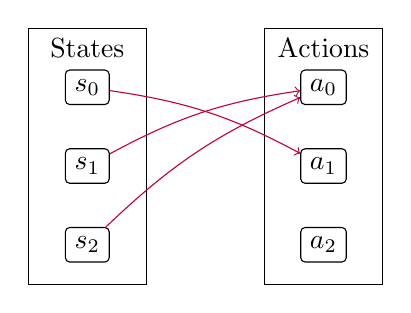
\begin{tikzpicture}
    \node[draw,rectangle,rounded corners=.55mm] (s0) at (0, 0) {$s_0$};
    \node[draw,rectangle,rounded corners=.55mm] (s1) at (0,-1) {$s_1$};
    \node[draw,rectangle,rounded corners=.55mm] (s2) at (0,-2) {$s_2$};
    \draw (-0.75, -2.5) rectangle (0.75, 0.75);
    \node at (0, 0.5) {States};
    \node[draw,rectangle,rounded corners=.55mm] (a0) at (3, 0) {$a_0$};
    \node[draw,rectangle,rounded corners=.55mm] (a1) at (3,-1) {$a_1$};
    \node[draw,rectangle,rounded corners=.55mm] (a2) at (3,-2) {$a_2$};
    \draw (2.25, -2.5) rectangle (3.75, 0.75);
    \node at (3, 0.5) {Actions};
    \path[->,purple] (s0) edge[bend left=10] (a1);
    \path[->,purple] (s1) edge[bend left=10] (a0);
    \path[->,purple] (s2) edge[bend left=10] (a0);
  \end{tikzpicture}
  \caption{\footnotesize We draw out a deterministic policy, which we denote by $\pi(s) = a$. In this example, the policy selects action $a_1$ in state zero, and action $a_1$ in states one and two. Notice that some actions are selected from more than one state, and that other actions are not selected at all.}
\end{figure}

\begin{table}[h]
  \centering
  \begin{tabular}{|c | c|}
    \hline
    State & Action \\
    \hline
    $s_0$ & $a_1$ \\
    \hline
    $s_1$ & $a_0$ \\
    \hline
    $s_2$ & $a_0$ \\
    \hline
  \end{tabular}
  \caption{\footnotesize A deterministic policy can also be represented by a table. Each row describes the action chosen by the policy $\pi$ in each state.}
\end{table}

\begin{figure}[h]
  \centering
  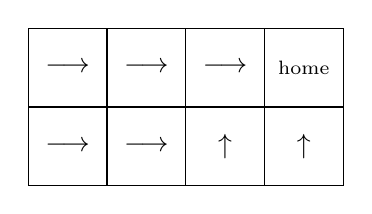
\begin{tikzpicture}
    \draw[step=1.0,black,thin] (0,0) grid (4, 2);
    \node at (3.5, 1.5) {\scriptsize home};
    \foreach \x in {0.5, 1.5} {
      \node at (\x, 0.5) {$\longrightarrow$};
      \node at (\x, 1.5) {$\longrightarrow$};
    }
    \node at (2.5, 0.5) {$\uparrow$};
    \node at (2.5, 1.5) {$\longrightarrow$};
    \node at (3.5, 0.5) {$\uparrow$};
  \end{tikzpicture}
  \caption{\footnotesize Consider a second deterministic policy in which an agent moves toward its home on a grid. The states correspond to the locations on the grid, and the actions move the agent up, down, left, and right. We've demarcated one possible policy using arrows. Each arrow tells the agent which direction to move in each state.}
\end{figure}

\paragraph{Stochastic Policies}
In general, a policy assigns probabilities to each action in each state; i.e. multiple actions may be selected each with some non-zero probability. If the agent is following policy $\pi$ at time $t$, then $\pi(a|s)$ is the probability that $A_t = a$ if $S_t = s$. Like $p$, $\pi$ is an ordinary function; the $|$ reminds us that it defines a conditional probability distribution over $a \in \mathcal A(s)$ for each $s \in \mathcal S$. Note that because $\pi(a|s)$ defines a probability distribution, we require that (i) $\sum_{a \in \mathcal A(s)} \pi(a|s) = 1$ and (ii) $\pi(a|s) \geq 0$.

\begin{figure}[h]
  \centering
  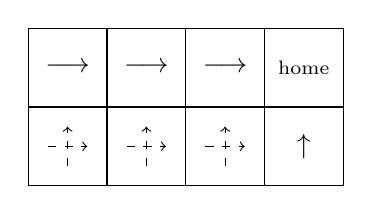
\begin{tikzpicture}
    \draw[step=1.0,black,thin] (0,0) grid (4, 2);
    \node at (3.5, 1.5) {\scriptsize home};
    \foreach \x in {0.5, 1.5} {
      \draw[->,dashed] (\x-.25, 0.5) -- (\x+.25, 0.5);
      \draw[->,dashed] (\x, 0.5-.25) -- (\x, 0.5+.25);
      \node at (\x, 1.5) {$\longrightarrow$};
    }
    \draw[->,dashed] (2.5-.25, 0.5) -- (2.5+.25, 0.5);
    \draw[->,dashed] (2.5, 0.5-.25) -- (2.5, 0.5+.25);
    \node at (2.5, 1.5) {$\longrightarrow$};
    \node at (3.5, 0.5) {$\uparrow$};    
  \end{tikzpicture}
  \caption{\footnotesize Here, we have a stochastic policy. We've indicated the randomness by drawing two possible actions with dashed lines for some of our states. To be concrete, the lower-left states each select an action of ``up'' or ``right'' each with probability $1/2$. Notice that the stochastic policy will require the \emph{same} number of steps to reach the house as the deterministic policy previously shown.}
\end{figure}

\subsubsection{(Action/State) Value Functions}
Many problems involve some sort of delayed reward; e.g. a store manager could lower their prices and sell off their entire inventory to maximize short-term gain. But, they might do better in the long-run by maintaining inventory to sell when demand is high. In RL, rewards capture the notion of short-term gains, but our objective is to learn a policy that achieves the most rewards in the long run; a value function formalizes what this means.

\paragraph{State value function}
The \emph{state-value function} of a state $s$ under a policy $\pi$, denoted by $v_\pi(s)$, is the expected return when starting in $s$ and following $\pi$ thereafter.\footnote{Note that because long-run outcomes depend on repeated actions and outcomes, value functions only make sense in the context of policies.} For MDPs, we can define this formally by
\begin{equation}
  \label{eq: statevalueforpolicypi}
  v_\pi(s) \coloneqq \mathbb E_{\pi} \left[ G_t | S_t = s \right] = \mathbb E_\pi \left[ \sum_{k=0}^{\infty} \gamma^k R_{t+k+1} | S_t = s \right], \hspace{24pt} \textrm{for all } s \in \mathcal S.
\end{equation}
We define the value of a terminal state (if there are any) to be zero. $v_\pi$ is the \emph{state-value function for policy $\pi$}. Crucially, value functions allow an agent to query the quality of its current situation as opposed to waiting to observe the long-term outcome; they summarize all possible futures by averaging over returns. Since ultimately we care about learning a good policy, the value function enables us to compare the quality of different policies!

\paragraph{Intuition on state-value functions} Suppose there is an agent playing a game of chess, which is clearly an episodic MDP. The state is given by the positions of all the pieces on the board, the actions are the set of legal moves, and termination occurs when the game ends in either a win, loss, or draw. We could define a reward as $+1$ when our agent wins and zero for all other moves. Realize that the reward doesn't tell us much about how well the agent is playing during the match: we have to wait till the end of the episode/game to realize the non-zero reward. However, the \emph{value function} lets us see much more; since the state value is equal to the expected sum of future rewards. In this case, we effectively defined reward as an indicator for winning, whence taking an expectation over an indicator variable we realize a probability, i.e. the value function in this instance encodes the probability of winning the game if we follow the policy $\pi$. Note that in this game, the opponent's move is part of the state transition. E.g. the environment moves both the agent's piece, and the opponent's piece, and this puts the board into a new state $s'$. An \emph{action-value function} would allow us to assess the probability of winning for each possible move given we follow the policy $\pi$ for the rest of the game.

\paragraph{Action value function}
We can also define the value of taking action $a$ in state $s$ under a policy $\pi$, denoted by $q_\pi(s,a)$, as the expected return starting from $s$, taking the action $a$, and thereafter following policy $\pi$:
\begin{equation}
  \label{eq: actionvaluepolicyforpi}
  q_\pi(s,a) \coloneqq \mathbb E_\pi \left[G_t | S_t = s, A_t = a \right] = \mathbb E_\pi \left[ \sum_{k=0}^\infty \gamma^k R_{t+k+1} | S_t = s , A_t = a \right].
\end{equation}
We refer to this as the \emph{action-value function for policy $\pi$}. Note that by the law of total probability, $v_\pi(s) = \mathbb E_\pi \left[G_t | S_t =       s\right] = \sum_{a} \pi(a|s) q_\pi(s,a)$.
We could also equivalently characterize the state-action function for a given policy $\pi$ by
\[
  q_\pi(s,a) = \sum_{s',r} \Pr(s', r | s, a) \left[ r + \gamma v_\pi (s') \right].
\]
\paragraph{Intuition for action value functions} Let's consider a continuing MDP.

\begin{figure}[h]
  \centering
  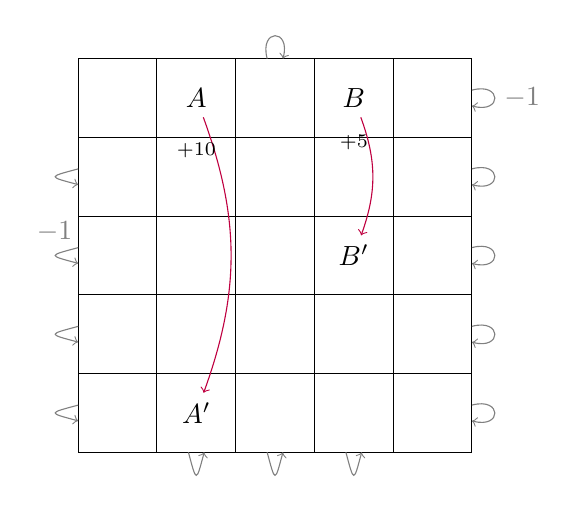
\begin{tikzpicture}
    \draw[step=1.0,black,thin] (0,0) grid (5, 5);
    \node (a) at (1.5, 4.5) {$A$};
    \node (ap) at (1.5, 0.5) {$A'$};
    \path[->,purple] (a) edge[bend left = 20] (ap);
    \node (b) at (3.5,4.5) {$B$};
    \node (bp) at (3.5, 2.5) {$B'$};
    \path[->,purple] (b) edge[bend left = 20] (bp);
    \node[below = 1mm of b] {$\scriptstyle +5$};
    \node[below = 2mm of a] {$\scriptstyle +10$};
    \foreach \x in {1.5, 2.5, 3.5} {
      \path[->] (\x-0.1, 0) edge[loop below,gray,distance=4mm] (\x+0.1, 0);
    }
    \path[->] (5, 4.6) edge[loop right,gray,distance=4mm] node[right] {$-1$}       (5, 4.4);
    \foreach \y in {3.5, 2.5, 1.5, 0.5} {
      \path[->] (5, \y+.1) edge[loop right,gray,distance=4mm] (5, \y-.1);
      \path[->] (0, \y+.1) edge[loop left ,gray,distance=4mm] (0, \y-.1);
    }
    \path[->] (2.4, 5) edge[loop above,gray,distance=4mm] (2.6, 5);
    \node[gray] at (-0.3, 2.8) {$-1$};
  \end{tikzpicture}
  \caption{\footnotesize The states are defined by the locations on the grid. The actions move the agent up, down, left, or right. The agent cannot move off the grid and bumping generates a reward of minus one. Most other actions yield no reward, but there are two special states labeled $A$ and $B$. Every action in state $A$ yields $+10$ reward and $+5$ in state $B$. Correspondingly, every action in $A$ and $B$ transition the agent with probability one to $A'$ and $B'$ respectively.}
\end{figure}

We must first specify the policy before we can figure out what the value function is. Suppose we start with a uniform random policy. Since this is a continuing task, we need to choose $\gamma < 1$. Let's try $\gamma = 0.9$.
We will later learn how to estimate the value function but for now let's take it as given below.

\begin{figure}[h]
  \centering
  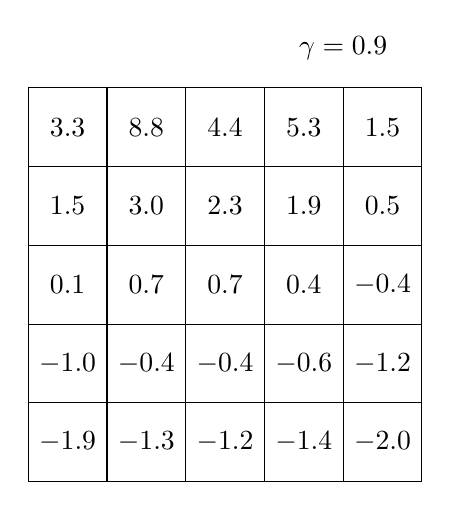
\begin{tikzpicture}
    \draw[step=1.0,black,thin] (0,0) grid (5, 5);
    % Bottom row
    \node at (0.5, 0.5) {$-1.9$};
    \node at (1.5, 0.5) {$-1.3$};
    \node at (2.5, 0.5) {$-1.2$};
    \node at (3.5, 0.5) {$-1.4$};
    \node at (4.5, 0.5) {$-2.0$};
    % Second to last row from bottom
    \node at (0.5, 1.5) {$-1.0$};
    \node at (1.5, 1.5) {$-0.4$};
    \node at (2.5, 1.5) {$-0.4$};
    \node at (3.5, 1.5) {$-0.6$};
    \node at (4.5, 1.5) {$-1.2$};
    % Middle row
    \node at (0.5, 2.5) {$0.1$};
    \node at (1.5, 2.5) {$0.7$};
    \node at (2.5, 2.5) {$0.7$};
    \node at (3.5, 2.5) {$0.4$};
    \node at (4.5, 2.5) {$-0.4$};
    % Second row from top
    \node at (0.5, 3.5) {$1.5$};
    \node at (1.5, 3.5) {$3.0$};
    \node at (2.5, 3.5) {$2.3$};
    \node at (3.5, 3.5) {$1.9$};
    \node at (4.5, 3.5) {$0.5$};
    % Top row
    \node at (0.5, 4.5) {$3.3$};
    \node at (1.5, 4.5) {$8.8$};
    \node at (2.5, 4.5) {$4.4$};
    \node at (3.5, 4.5) {$5.3$};
    \node at (4.5, 4.5) {$1.5$};
    % Gamma factor for clarity.
    \node at (4, 5.5) {$\gamma = 0.9$};
  \end{tikzpicture}
  \caption{\footnotesize Recall that we have simulated a value function for an agent under a random action policy. Notice the negative values near the bottom, these values are low because the agent is likely to bump into the wall before reaching the distant states $A$ or $B$. Remember that $A$ and $B$ are both the only sources of positive reward in this MDP. It's interesting to note that the state-value function at $A$ is $<10$, even though the immediate reward is $+10$: because every transition from $A$ moves the agent closer to the lower wall in which the random policy is likely to bump and get a negative reward. I.e. in expectation the reward is slightly less than $+10$ because we expect to also run into a wall. On the other hand, the state-value at $B$ is slightly greater than $+5$, because the next step involves moving the agent to the middle of the grid where they are unlikely to bump into any edges and further its reasonably close to states $A$ and $B$. The value function compactly summarizes all these possibilities.}
\end{figure}

``The essence of reinforcement learning is combining search with memory'' -Rich Sutton. ``RL at its root is memoized (context-sensitive) search'' -Andy Barto.

\paragraph{Monte Carlo methods} We can estimate $v_\pi$ and $q_\pi$ from experience. If an agent follows policy $\pi$ and maintains an average, for each state encountered, of the actual returns that have followed that state, then the average will converge to the state's value $v_\pi(s)$ as the number of times that state is encountered approaches infinity. If separate averages are kept for each action taken at each state, then these averages will similarly converge to the action values $q_\pi(s,a)$. Methods of estimating in this way are known as Monte Carlo methods because they involve averaging over many random samples of actual returns. If there are very many states, it many not be practical to keep separate averages for each state individually. Instead, we could have our agent maintain $v_\pi$ and $q_\pi$ as parameterized functions (with fewer parameters than states), and adjust the parameters to match the observed returns; these are known as approximate solution methods.

\paragraph{Bellman equation for state-value function}
In everyday life, we learn a lot without getting explicit positive or negative feedback. E.g. you could be riding your bike and hit a rock that sends you off balance. In spite of not getting injured, you learn to avoid rocks in the future and perhaps react more quickly if you do it one. How do we know that hitting a rock is bad even when nothing bad happened \emph{this} time? The answer is that we recognize that losing our balance is bad even without falling and hurting ourselves, and perhaps we've had similar experiences in the past when things didn't work out so nicely. In RL, there's a similar idea that allows us to relate the value of the current state to the value of future states without waiting to observe all future rewards: we use the Bellman equations to formalize this connection between the value of a state and its possible successors.
For any policy $\pi$ and any state $s$, the following consistency condition holds between the value of $s$ and the value of its possible successor states:
\begin{align}
  v_\pi(s) &\coloneqq \mathbb E_\pi \left[ G_t | S_t = s \right] \nonumber \\
           &= \color{purple} \mathbb E_\pi \left[ \color{orange} R_{t+1} + \gamma G_{t+1} \color{purple} | S_t = s \right] &\textrm{by equation } \ref{eq: recursivereturnformulation} \nonumber  \\
           &= \color{purple} \sum_a \pi(a|s) \sum_{s'} \sum_{r} \Pr(s',r|s,a) \left[ \color{orange} r + \gamma                           \underbrace{\mathbb E_\pi \left[G_{t+1} | S_{t+1} = s' \right]}_{v_*(s')} \color{purple} \right] \nonumber  \\
  \label{eq: bellmaneqforstatevaluepolicy}
           &= \sum_a \pi(a|s) \sum_{s',r} \Pr(s',r|s,a) \left[r + \gamma v_\pi(s')\right], \hspace{25pt} \textrm{for all } s \in \mathcal S.
\end{align}
The penultimate equality follows from the definition of expectation in two steps (the first step is to integrate out all possible actions, and the second is to integrate over all possible rewards and next states), and all we're doing is writing out our expectation explicitly as a weighted sum of possible outcomes, where the weights are the probabilities the event occurs. Note that we could continue to recursively expand our expression, but this would only make it more complicated. Further, realize that embedded in our expression is the value function for state $s'$, i.e. $v_*(s')$, with the only difference being that the time index is time step $t+1$ instead of $t$. But, realize that neither the policy nor $p$ depends on time. Making this replacement, we realize the Bellman equation for the state-value function. I.e. equation \ref{eq: bellmaneqforstatevaluepolicy} is known as the Bellman equation for $v_\pi$: it expresses a relationship between the value of a state and the values of its successor states. The magic value is that we can use them as a stand-in for the average of an infinite number of possible futures.

\begin{figure}[h]
  \centering
  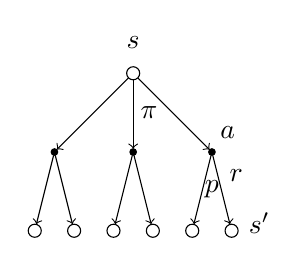
\begin{tikzpicture}
    \node[draw,circle,scale=1/2] (s) at (0,0) {};
    \node[above=1mm of s] {$s$};
    \foreach \x in {-1, 0, 1} {
      \node[draw,circle,fill,scale=1/4] (b\x) at (\x, -1) {};
      \node[draw,circle,scale=1/2] (l\x) at (\x-.25,-2) {};
      \node[draw,circle,scale=1/2] (r\x) at (\x+.25,-2) {};
      \draw[->] (s) -- (b\x);
      \draw[->] (b\x) -- (l\x);
      \draw[->] (b\x) -- (r\x);
    }
    \node at (0.2, -0.5) {$\pi$};
    \node at (1.2, -0.75) {$a$};
    \node[below = 2mm of b1] {$p$};
    \node[below right = 1mm of b1] {$r$};
    \node at (1.6, -1.9) {$s'$};
  \end{tikzpicture}
\caption{\footnotesize Think of looking ahead from a state to its possible successor states. Each open circle represents a state, and each solid circle represents a state-action pair. Starting from state $s$, the root node, the agent can take ay of some set of actions (three of which are shown in the diagram) based on its policy $\pi$. From each of these, the environment could respond with one of several next states, $s'$ (two are shown in the figure), along with a reward $r$, depending on the dynamics given by the function $p$. The Bellman equation \ref{eq: bellmaneqforstatevaluepolicy} averages over all possibilities, weighting each by its probability of occurring. It states that the value of the start state must equal the discounted value of the expected next state, plus the reward expected along the way.}
\label{fig: bellmanlookahead}
\end{figure}

If $r(s,a)$ is the expected reward for taking action $a$ in state $s$, then we can re-express the Bellman equations using this expected reward function as follows.
\begin{align*}
  q_\pi(s,a) &= r(s,a) + \gamma \sum_{s', a'} \Pr(s' | s, a) \pi(a'|s')                q_\pi(s',a') \\
  v_\pi(s) &= \sum_a \pi(a|s) \left[r(s,a) + \gamma \sum_{s'} \Pr(s'|s,a)              v_\pi(s')\right] \\
  v_*(s) &= \max_a \left[r(s,a) + \gamma \sum_{s'} \Pr(s'|s,a) v_*(s')\right].
\end{align*}

The value function $v_\pi$ is the unique solution to its Bellman equation. Diagrams like \ref{fig: bellmanlookahead} are called \emph{backup diagrams} because they diagram relationships that form the basis of the \emph{update} operations; these operations transfer value information \emph{back} to a state (or state-action pair) from its successor states (or state-action pairs). Unlike transition graphs, the state nodes of backup diagrams do not necessarily represent distinct states, e.g. a state might be its own successor.

\paragraph{Action-value Bellman equation}
We can derive a similar equation for the action-value function. It will be a recursive equation for the value of a state-action pair in terms of its possible successor state-action pairs. In this case, the equation does not begin with the policy selecting an action: this is because the action is already fixed as part of the input argument state-action pair. Instead, we simply skip to the dynamics function $p$ which selects the immediate reward and next state $s'$. Again, we have a weighted sum over terms consisting of immediate reward plus expected future return given a specific next state little $s'$. Unlike the Bellman equation for the state value function, we can't stop here. We want a recursive equation for the value of one state-action pair in terms of the \emph{next} state-action pair. 
\begin{align}
  q_\pi(s,a) &\coloneqq \color{purple} \mathbb E_\pi \left[ \color{black} G_t                \color{purple} | S_t = s, A_t = a \right] \\
             &= \color{purple} \sum_{s'} \sum_{r} \Pr(s', r | s, a) \color{black} \left[r + \gamma \color{orange} \mathbb E_\pi \left[G_{t+1} | S_{t+1} = s' \right] \color{black} \right]
\end{align}
At the moment we have the expected return given only the next state. To change this, we can express the expected return from the next state as a sum of the agent's possible action choices, via law of total probability. In particular, we can change the expectation to be conditioned on both the next state and the next action and then sum over all possible actions.
\begin{align*}
  &= \sum_{s'} \sum_{r} \Pr(s', r|s,a) \left[ r + \gamma \color{orange} \sum_{a'} \pi(a'|s') \mathbb E_\pi \left[G_{t+1} | S_{t+1} = s', A_{t+1} = a' \right] \color{black} \right]
\end{align*}
Each term is weighted by the probability under our policy $\pi$ of selecting $a'$ in the state $s'$. This expected return is the same as the definition of the action-value function for $s'$ and $a'$. Making this replacement, we get the Bellman equation for the action-value function.
\begin{align*}
  &= \sum_{s'} \sum_{r} \Pr(s', r|s,a) \left[ r + \gamma \sum_{a'} \pi(a'|s')\color{orange} q_\pi(s',a') \color{black} \right]
\end{align*}

Bellman equations for both state and action-value functions provide relationships between the values of a state or state-action pair and the possible next states or next state-action pairs. These equations capture an important structure of the RL problem, and we will discuss how we can use this to design algorithms which efficiently estimate value functions.

\paragraph{Using Bellman equations to compute value-functions} Let's illustrate a simple example consisting of four states, labeled $A$, $B$, $C$, and $D$ on a grid. The action space consists of moving up, down, left, and right. Actions which would move off the grid, instead keep the agent in place. E.g. if we start in state $C$ and move ``up'' we end in state $A$. If we then try to move ``left'' we would hit a wall and stay in state $A$. MOve to the right next would take us to state $B$, etc. The reward is $0$ everywhere except for any time the agent lands in state $B$, in which case it gets a reward of $+5$; this includes starting in state $B$ and hitting a wall to remain there.
\begin{figure}[h]
  \centering
  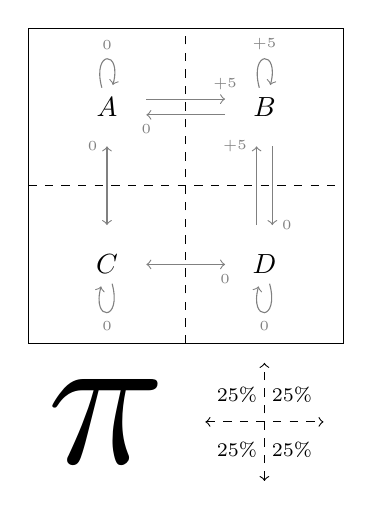
\begin{tikzpicture}
    \draw[step=2.0,black,thin, dashed] (0,0) grid (4, 4);
    \draw (0, 0) rectangle (4, 4);
    \node (a) at (1, 3) {$A$};
    \node (b) at (3, 3) {$B$};
    \node (c) at (1, 1) {$C$};
    \node (d) at (3, 1) {$D$};
    % States A-B
    \draw[->,gray] (1.5, 3.1) -- (2.5, 3.1) node[above, gray] {\tiny +5};
    \draw[->,gray] (2.5, 2.9) -- (1.5, 2.9) node[below, gray] {\tiny 0};
    % States B-D
    \draw[->,gray] (2.9, 1.5) -- (2.9, 2.5) node[left, gray] {\tiny +5};
    \draw[->,gray] (3.1, 2.5) -- (3.1, 1.5) node[right, gray] {\tiny 0};
    % States C-D
    \draw[<->,gray] (1.5, 1) -- (2.5, 1) node[below,gray] {\tiny 0};
    % States A-C
    \draw[<->,gray] (1, 1.5) -- (1, 2.5) node[left,gray] {\tiny 0};
    % Self-loops.
    \path[gray] (a) edge[loop above] node[above] {\tiny 0} (a);
    \path[gray] (b) edge[loop above] node[above] {\tiny +5} (b);
    \path[gray] (c) edge[loop below] node[below] {\tiny 0} (c);
    \path[gray] (d) edge[loop below] node[below] {\tiny 0} (d);
    % Policy
    \node at (1,-1) {\resizebox{1.5cm}{!}{$\pi$}};
    \draw[<->,dashed] (2.25, -1) -- (3.75, -1);
    \draw[<->,dashed] (3, -1.75) -- (3, -0.25);
    \node at (3.35, -0.65) {\scriptsize 25\%};
    \node at (2.65, -0.65) {\scriptsize 25\%};
    \node at (2.65, -1.35) {\scriptsize 25\%};
    \node at (3.35, -1.35) {\scriptsize 25\%};
  \end{tikzpicture}
\end{figure}
Suppose we consider a uniform random policy, which moves in each direction $1/4$ of the time. Since this is a continuing task, we choose a discount factor of $\gamma = 0.7$. How can we actually work out the value of each of these states under this policy?  Recall that the value function is the expected return under policy $\pi$, i.e. an average over the return obtained by each sequence of actions an agent could possibly choose (infinitely many possible futures). Fortunately, the Bellman equation for the state-value function provides an elegant solution: using the Bellman equation, we can write down an expression for the value of state $A$ in terms of the sum of the four possible actions the resulting possible successor states.

\begin{equation*}
  v_\pi(s) = \color{purple} \sum_a \pi(a|s) \color{orange} \sum_r \sum_{s'} \color{black} \Pr(\left(s', r|s,a\right) \left[ \color{orange} r + \gamma v_\pi(s') \color{black} \right]
\end{equation*}
We can simplify the expression further \emph{in this case}, because for each action there's only one possible associated next state and reward,
i.e. the sum over $s'$ and $r$ reduces to a single value.
\[
v_\pi(A) = \color{purple} \sum_a \pi(a|A) \color{orange} \left(r + 0.7 v_\pi(s')\right)
\]
To go even further, if we go right from state $A$, we land in state $B$ and receive a reward of $+5$. This happens $1/4$ of the time under the random policy. If we go down, we land in state $C$, and receive no immediate reward, and this occurs $1/4$ of the time. If we go either up or left, we will land back in state $A$ again, since each of the actions occur with probability $1/4$, and since both actions land back in state $A$ and receive no reward, we can combine them into a single term with a coefficient of $1/2$.
\[
  v_\pi(A) = \color{purple} \frac{1}{4} \color{orange} \left(5 + 0.7 v_\pi(B)\right) \color{black} + \color{purple} \frac{1}{4} \color{orange} \left(0.7 v_\pi(C)\right) \color{black} + \color{purple} \frac{1}{2} \color{orange} 0.7 v_\pi(A).
\]
Using the same methodology, we can write down a similar equation for each of the other states.
\begin{align*}
  v_\pi(B) &= \frac{1}{2} \left(5 + 0.7 v_\pi(B)\right) + \frac{1}{4} 0.8              v_\pi(A) + \frac{1}{4} 0.7 v_\pi (D) \\
  v_\pi(C) &= \frac{1}{4} 0.8 v_\pi(A) + \frac{1}{4} 0.8 v_\pi(D) + \frac{1}{2}              0.7 v_\pi(C) \\
  v_\pi(D) &= \color{purple} \frac{1}{4} \color{orange} \left(5 + 0.7 V_\pi(B)\right) \color{black} + \color{purple} \frac{1}{4} \color{orange} 0.7 v_\pi(C) \color{black} + \color{purple} \frac{1}{2} \color{orange} 0.7 v_\pi(D).
\end{align*}
We now have a system of four equations in four unknowns, which can be solved for. The unique solution for this example happens to work out to
\[
  v_\pi(A) = 4.2, \hspace{15pt} v_\pi(B) = 6.1, \hspace{15pt} v_\pi(C) = 2.2, \hspace{15pt} v_\pi(D) = 4.2.
\]
What's important to note is that the Bellman equation reduced an unmanageable infinite sum over possible futures to a simple linear algebra problem. The Bellman equation provides a powerful general relationship for MDPs.
Note that for more interesting problems like chess, we won't even be able to list all possible states, since there are around $10^{45}$ of them, let alone construct and solve the resulting system of Bellman equations.

\subsection{Optimal Policies and Optimal Value Functions}
Up to this point, we've generally talked about a policy as something that is given; it specifies how our agent behaves. Given such a way of behaving, we've discussed how to find the value function. 
But, solving an RL task means \emph{finding} a policy that achieves a lot of reward over the long run. For finite MDPs, we can precisely find an optimal policy as follows. Value functions define a partial ordering over policies: a policy $\pi$ is defined to be better than or equal to another policy $\pi'$ if its expected return is greater than or equal to that of $\pi'$ for all states. I.e. $\pi \geq \pi' \iff v_\pi(s) \geq v_{\pi'}(s)$ for all $s \in \mathcal S$.
If a policy is better than another in some states but not others, we cannot say that one policy is better than the other. Clearly, there is always at least one policy that is better than or equal to all other policies; this is an \emph{optimal policy}.\footnote{To see this, suppose that we have two policies $\pi_1$ and $\pi_2$, where $\pi_1$ sees some states with higher value relative to $\pi_2$, but not for all states. We can create a new policy $\pi_3$ which is defined by combining the two aforementioned policies such that for each state we select the policy that performs best. This new policy $\pi_3$ will have a value greater than or equal to both $\pi_1$ and $\pi_2$ in \emph{every} state. Therefore, we will never have a situation where doing well in one state requires a sacrifice at another. Due to this (informal) reasoning, there will always exist some policy which is best in every state. Note that it's possible that $\pi_3$ achieves values that strictly exceed both of $\pi_1$ and $\pi_2$, and this is due to the fact that by playing other states more optimally that are closeby, we could be setting ourselves up for a higher long-term reward.} Although there may be more than one, we denote all optimal policies by $\pi_*$.

\paragraph{Example optimal policy}
Let's consider a two-choice MDP, where the only decision to be made is in the top state labeled $X$.
\begin{figure}[h]
  \centering
  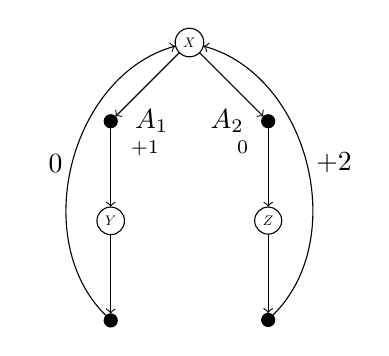
\begin{tikzpicture}
    \node[draw,circle,scale=1/2] (x) at (0, 0) {$X$};
    \node[draw,circle,fill,scale=1/2] (a1) at (-1, -1) {};
    \node[draw,circle,fill,scale=1/2] (a2) at ( 1, -1) {};
    \node[draw,circle,below=1cm of a1,scale=1/2] (y) {$Y$};
    \node[draw,circle,below=1cm of a2,scale=1/2] (z) {$Z$};
    \node[draw,circle,fill,scale=1/2,below=1cm of y] (l) {};
    \node[draw,circle,fill,scale=1/2,below=1cm of z] (r) {};
    \draw[->] (x) -- (a1);
    \draw[->] (x) -- (a2);
    \draw[->] (a1) -- (y);
    \draw[->] (a2) -- (z);
    \node[below right = 1mm of a1] {\scriptsize +1};
    \node[below left  = 1mm of a2] {\scriptsize 0};
    \draw[->] (y) -- (l);
    \draw[->] (z) -- (r);
    \path[->] (l) edge[bend left=60] node[left] {0} (x);
    \path[->] (r) edge[bend right=60] node[right] {+2} (x);
    \node[right = 1mm of a1] {$A_1$};
    \node[left = 1mm of a2] {$A_2$};
  \end{tikzpicture}
  \caption{\footnotesize The agent can take either action $A_1$ or $A_2$. From state $X$, action $A_1$ takes the agent to state $Y$. In state $Y$, only action $A_1$ is available and it takes the agent back to $X$. On the other hand, action $A_2$ (from $X$) takes the agent to state $Z$. From state $Z$, action $A_1$ is again the only action available and it takes the agent back to state $X$. Realize that although action $A_1$ gives an immediate reward of $+1$, action $A_2$ offers a larger (albeit delayed) reward of $+2$ after a single step delay.}
\end{figure}
In the above MDP, there are only two deterministic policies which are completely defined by the agent's choice in state $X$: take action $A_1$ or action $A_2$. Let's call these $\pi_1$ and $\pi_2$ respectively.
\[
  \pi_1(X) = A_1, \hspace{25pt} \pi_2(X) = A_2.
\]
The optimal policy is the one for which the value of $X$ is highest, but the answer depends on the discount factor $\gamma$ (since this is a continuing task). If $\gamma = 0$, then the value function is defined using only the \emph{immediate} reward. In this case, the value of $X$ under $\pi_1$ is $+1$, while the value under $\pi_2$ is zero because the positive reward is only incurred after a delay, and this doesn't affect the return when $\gamma = 0$. In this case of $\gamma = 0$, then $\pi_1$ is the optimal policy. What if instead, $\gamma = 0.9$? In this case, the value of $X$ under each policy is an infinite sum. The state-value functions are
\begin{align*}
  v_{\pi_1}(X) &= 1 + 0.9 * 0 + (0.9)^2 * 1 + \ldots = \sum_{k=0}^{\infty} 0.9^{2k} = \frac{1}{1-0.9^2} \approx 5.3 \\
  v_{\pi_2}(X) &= 0 + 0.9 * 2 + (0.9)^2 * 0 + \ldots = \sum_{k=0}^{\infty} (0.9)^{2k+1}*2 = \frac{0.9}{1-0.9^2} * 2 \approx 9.5
\end{align*}
We've used the fact that we can compactly represent each state-value function by a geometric series. Note that in the case of $\pi_1$, we are incurring a positive unit valued reward on each even time step, whereas for $\pi_2$ we are incurring a slightly higher reward on each odd time step. In this example, $\pi_2$ is the more optimal policy, and we could find it simply by computing the state-value function for each deterministic policy under consideration.\footnote{As a final example consider the case of $\gamma = 0.5$.In this case, $v_{\pi_1} = \frac{1}{1-0.5^2} = \frac{4}{3}$ and $v_{\pi_2} = \frac{0.5}{1 - 0.5^2} \times 2 = \frac{4}{3}$ and both policies are optimal.}
In general, it won't be so easy. Even if we limited ourselves to deterministic policies, the number of possible policies is equal to the number of possible actions raised to the number of possible states, $|\mathcal A|^{|\mathcal S|}$. This means we cannot use a brute force search for even moderately sized problems. Fortunately, the \emph{Bellman optimality equations} can help us organize our search of the policy space.

\paragraph{Optimal value functions}
Optimal policies achieve the goal of RL by achieving as much reward as possible in the long run, but the exponential number of possible policies make searching for the optimal policy by brute-force intractable.
Recall that
\[
  \pi_1 \geq \pi_2 \iff v_{\pi_1}(s) \geq v_{\pi_2}(s) \hspace{10pt} \forall \hspace{10pt} s \in \mathcal S.
\]
An optimal policy is one that is as good or better than every other policy. The value function for the optimal policy thus has the greatest value possible in every state.
\begin{align*}
  v_{\pi_*}(s) \coloneqq \mathbb E_{\pi_*} \left[ G_t | S_t = s \right] = \max_\pi v_\pi (s) \hspace{10pt} \forall \hspace{5pt} s \in \mathcal S.
\end{align*}
What does it mean to take a maximum over different policies? Imagine we were to consider every possible policy and compute each of their values for the state $s$: the value of an optimal policy is defined to be the largest of all the computed values. We could repeat this for every state and the value of an optimal policy would always be largest. 

\paragraph{Optimal Policies}
An optimal policy is defined as the policy with the highest possible value function in all states. At least one optimal policy always exists, but there may be more than one.
They share the same state-value function, called the \emph{optimal state-value function}, denoted $v_*$, and defined as
\[
  v_*(s) = \max_\pi v_\pi(s)
\]
for all $s \in \mathcal S$. Note that optimal policies also share the same \emph{optimal action-value function}, denoted $q_*$, and defined as
\[
  q_*(s,a) = \max_\pi q_\pi(s,a),
\]
for all $s \in \mathcal S$ and $a \in \mathcal A(s)$. For the state-action pair $(s,a)$, this function gives the expected return for taking action $a$ in state $s$ and thereafter following an optimal policy. Thus, we may write $q_*$ in terms of $v_*$ as follows:
\[
  q_*(s,a) = \mathbb E \left[ R_{t+1} + \gamma v_*(S_{t+1}) | S_t = s, A_t = a \right].
\]
\paragraph{Bellman optimality equation}
Because $v_*$ is the value function for \emph{a} policy, it must satisfy the self-consistency condition given by the Bellman equation \ref{eq:   bellmaneqforstatevaluepolicy} for state values. I.e. we have that
\[
  v_\pi(s) = \sum_a \pi(a|s) \sum_{s'} \sum_r \Pr(s', r | s, a) \left[ r + \gamma v_\pi(s')\right].
\]
If we simply substitute the optimal policy $\pi_*$ into this equation, we get the Bellman equation for $v_*$,
\[
  \color{purple} v_*(s) \color{black} = \sum_a \color{orange} \pi_* \color{black} (a|s) \sum_{s'} \sum_r \Pr(s', r | s, a) \left[ r + \gamma \color{purple} v_* \color{black} (s') \right].
\]
So far, nothing special, we've simply substituted an optimal policy into the Bellman equation. However, because this is an optimal policy, $v_*$ can be written in a special form without referencing the policy itself. Remember that there always exists an optimal deterministic policy, one that selects an optimal action in every state. Such a determinstic policy would assign probability 1 for an action that achieves the highest value and probability zero for all other actions. We can express this another way by replacing the sum over $\pi_*$ with a maximum over the action-space, i.e. using $\max_a$:
\begin{equation}
  \label{eq: bellmanoptimalityequationforvstar}
\color{purple} v_* \color{black} (s) = \color{purple} \max_{\color{black} a} \color{black} \sum_{s'} \sum_r \Pr(s', r | s,a) \left[ r + \gamma \color{purple} v_* \color{black}(s')\right].
\end{equation}
Notice that $\pi_*$ no longer appears in the equation! We have derived a relationship that applies directly to $v_*$ itself. This 
special form of the equation is known as the \emph{Bellman optimality equation} for $v_*$. Intuitively, this equation expresses the fact that the value of a state under an optimal policy \emph{must equal} the expected return for the best action from that state; re-writing it all together:
\begin{align}
  v_*(s) &= \max_{a \in \mathcal A(s)} q_{\pi_*} (s,a) = \max_a \mathbb E_{\pi_*} \left[G_t | S_t = s, A_t = a \right] = \max_a \mathbb E_{\pi_*} \left[R_{t+1} +            \gamma G_{t+1} | S_t = s, A_t = a \right] \nonumber \\
         &= \max_a \mathbb E \left[R_{t+1} + \gamma v_*(S_{t+1}) | S_t = s, A_t                       = a \right] \\
  \label{eq: bellmanoptimalityequationforpi}
         &= \max_a \sum_{s',r} \Pr(s', r|s,a) \left[r + \gamma v_*(s')\right].
\end{align}
The last two equations are just two different forms of the Bellman optimality equation for $v_*$.
\begin{figure}[h]
  \centering
  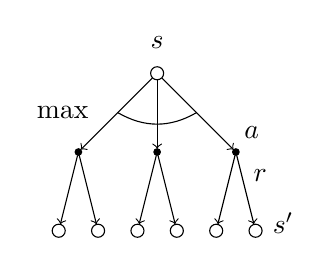
\begin{tikzpicture}
    \node[draw,circle,scale=1/2] (s) at (0,0) {};
    \node[above=1mm of s] {$s$};
    \foreach \x in {-1, 0, 1} {
      \node[draw,circle,fill,scale=1/4] (b\x) at (\x, -1) {};
      \node[draw,circle,scale=1/2] (l\x) at (\x-.25,-2) {};
      \node[draw,circle,scale=1/2] (r\x) at (\x+.25,-2) {};
      \draw[->] (s) -- (b\x);
      \draw[->] (b\x) -- (l\x);
      \draw[->] (b\x) -- (r\x);
    }
    % \node at (0.2, -0.5) {$\pi$};
    \node at (1.2, -0.75) {$a$};
    % \node[below = 2mm of b1] {$p$};
    \node[below right = 1mm of b1] {$r$};
    \node at (1.6, -1.9) {$s'$};
    \node at (-1.2, -0.5) {max};
    \path[-] (-.5,-.5) edge[bend right=30] (.5, -.5);
  \end{tikzpicture}
  \caption{\footnotesize We draw a backup diagram for the Bellman optimality equation \ref{eq: bellmanoptimalityequationforpi} for $v_*$. Notice that we've added an arc to indicate that the agent's choice points to represent that the maximum over that choice is taken rather than the expected value given some policy.}
\end{figure}

\paragraph{Bellman \emph{optimality} equation for action-value function}
The Bellman optimality equation for $q_*$ can be derived in a similar way, where we replace a summation over actions by a maximum, using a similar argument as above. Recall that
\[
q_\pi(s,a) = \sum_{s'} \sum_r\Pr(s', r|s,a) \left[ r + \gamma \sum_{a'} \pi(a',s')q_\pi(s',a')\right]
\]
and we can substitute in an optimal policy to yield
\[
  \color{purple} q_* \color{black} (s,a) = \sum_{s'} \sum_r \Pr(s',r|s,a) \left[ r + \gamma \sum_{a'} \color{orange} \pi_* \color{black} (a'|s') \color{purple} q_* \color{black}(s',a')\right].
\]
Making a similar argument as above, we can replace the use of a probability distribution $\pi_*(a',s')$ with a call to $\max_{a'}$, since our policy is optimal:
\[
  \color{purple} q_* \color{black} (s,a) = \sum_{s'} \sum_r \Pr(s',r|s,a) \left[ r + \gamma \underbrace{\color{purple} \max_{a'} \color{purple} q_* \color{black}(s',a')}_{=v_*(s')}\right].  
\]
This yields the Bellman optimality equation for $q_*$. Writing it all out again in slightly different notation:
\[
  q_*(s,a) = \mathbb E \left[R_{t+1} + \gamma \max_{a'} q_*(S_{t+1}, a') | S_t = s, A_t = a \right] = \sum_{s',r} \Pr(s', r|s,a) \left[r + \gamma \max_{a'} q_*(s', a') \right].
\]
We discussed previously that the Bellman equations allowed us to form a linear system of equations for which we could solve for the value-state functions. The Bellman optimality equation gives us a similar system of equations for the \emph{optimal} value.
\begin{figure}[h]
  \centering
  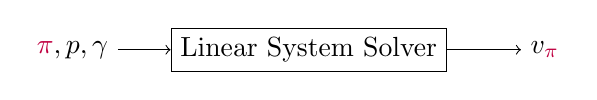
\begin{tikzpicture}
    \node (math) at (0,0) {$\color{purple} \pi \color{black}, p, \gamma$};
    \node[draw,rectangle] (solver) at (3,0) {Linear System Solver};
    \node (v) at (6, 0) {$v_{\color{purple}\pi}$};
    \draw[->] (math) -- (solver);
    \draw[->] (solver) -- (v);
  \end{tikzpicture}
  \caption{\footnotesize A simple diagram showing how we can use a policy to determine a value-function.}
\end{figure}
One natural question is: can we solve this system in a similar way to find the optimal state-value function? Unfortunately, no, since the $\max$ operation over actions is not linear! Standard techniques from linear algebra no longer apply. In this course, we'll use other techniques based on the Bellman equations to compute value functions and policies. We might also wonder why we can't simply use $\pi_*$ in the ordinary Bellman equation to get a system of linear equations for $v_*$, but unfortunately we don't know $\pi_*$ (learning \emph{it} is the fundamental goal of RL).

\begin{figure}[h]
  \centering
  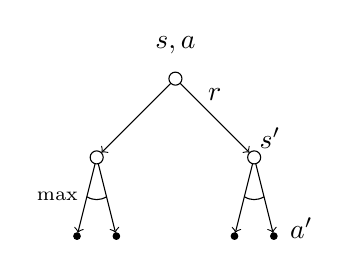
\begin{tikzpicture}
    \node[draw,circle,scale=1/2] (s) at (0,0) {};
    \node[above=1mm of s] {$s,a$};
    \node at (0.5, -0.2) {$r$};
    \foreach \x in {-1, 1} {
      \node[draw,circle,scale=1/2] (b\x) at (\x, -1) {};
      \node[draw,circle,fill,scale=1/4] (l\x) at (\x-.25,-2) {};
      \node[draw,circle,fill,scale=1/4] (r\x) at (\x+.25,-2) {};
      \draw[->] (s) -- (b\x);
      \draw[->] (b\x) -- (l\x);
      \draw[->] (b\x) -- (r\x);
      \path[-] (\x+.125,-1.5) edge[bend left=30] (\x-.125,-1.5);
    }
    \node at (-1.5, -1.5) {\scriptsize max};
    \node at (1.2, -0.75) {$s'$};
    % \node[below = 2mm of b1] {$p$};
    \node at (1.6, -1.9) {$a'$};
    % \node at (-1.2, -0.5) {max};
    % \path[-] (-.5,-.5) edge[bend right=30] (.5, -.5);
  \end{tikzpicture}
  \caption{\footnotesize We draw a backup diagram for the Bellman optimality equation for $q_*$.}
\end{figure}

\paragraph{Uniqueness of solution for value function}
For finite MDPs, the Bellman optimality equation for $v_*$ has a unique solution: it's actually a system of equations (one for each state), so if there are $n$ states or equations then there are also $n$ unknowns. If the dynamics $p$ of the environment are known, then in principle one can solve this system of equations for $v_*$ using any one of a variety of methods for solving systems of \emph{nonlinear} equations. We can also solve a related set of equations for $q_*$.

\paragraph{Using $v_*$ to determine an optimal policy}
Having learned about optimal value functions and the Bellman optimality equations, we might wonder why this all matters when our ultimate goal is not to find the \emph{value function} of an optimal policy but instead just the optimal policy itself! It turns out it's quite easy to go from an optimal value function to the associated optimal policy; the two goals are almost the same.
Let us return to our grid-world problem from before.

\begin{figure}[h]
  \centering
    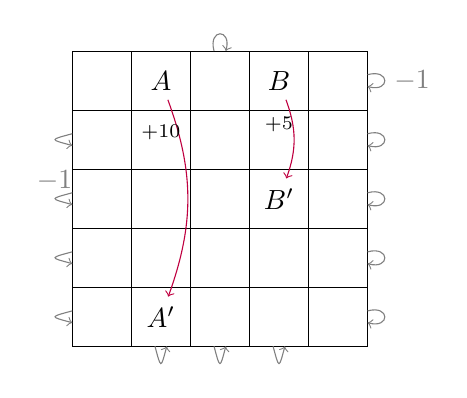
\begin{tikzpicture}[scale=0.75]
    \draw[step=1.0,black,thin] (0,0) grid (5, 5);
    \node (a) at (1.5, 4.5) {$A$};
    \node (ap) at (1.5, 0.5) {$A'$};
    \path[->,purple] (a) edge[bend left = 20] (ap);
    \node (b) at (3.5,4.5) {$B$};
    \node (bp) at (3.5, 2.5) {$B'$};
    \path[->,purple] (b) edge[bend left = 20] (bp);
    \node[below = 1mm of b] {$\scriptstyle +5$};
    \node[below = 2mm of a] {$\scriptstyle +10$};
    \foreach \x in {1.5, 2.5, 3.5} {
      \path[->] (\x-0.1, 0) edge[loop below,gray,distance=4mm] (\x+0.1, 0);
    }
    \path[->] (5, 4.6) edge[loop right,gray,distance=4mm] node[right] {$-1$}       (5, 4.4);
    \foreach \y in {3.5, 2.5, 1.5, 0.5} {
      \path[->] (5, \y+.1) edge[loop right,gray,distance=4mm] (5, \y-.1);
      \path[->] (0, \y+.1) edge[loop left ,gray,distance=4mm] (0, \y-.1);
    }
    \path[->] (2.4, 5) edge[loop above,gray,distance=4mm] (2.6, 5);
    \node[gray] at (-0.3, 2.8) {$-1$};
  \end{tikzpicture}
\end{figure}

Let's hold off on the question of how to find an optimal value function, but instead take the associated optimal values for each state as given.

\begin{figure}[h]
  \centering
    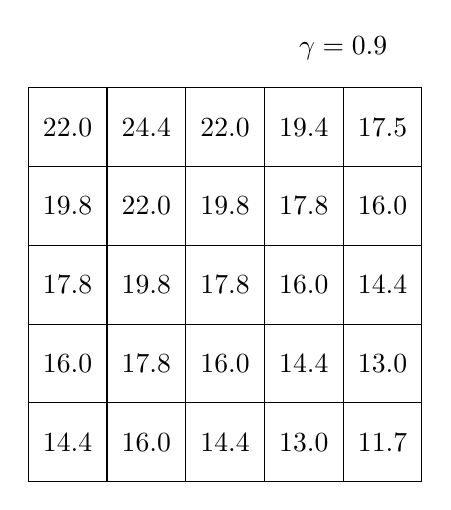
\begin{tikzpicture}
    \draw[step=1.0,black,thin] (0,0) grid (5, 5);
    % Bottom row
    \node at (0.5, 0.5) {$14.4$};
    \node at (1.5, 0.5) {$16.0$};
    \node at (2.5, 0.5) {$14.4$};
    \node at (3.5, 0.5) {$13.0$};
    \node at (4.5, 0.5) {$11.7$};
    % Second to last row from bottom
    \node at (0.5, 1.5) {$16.0$};
    \node at (1.5, 1.5) {$17.8$};
    \node at (2.5, 1.5) {$16.0$};
    \node at (3.5, 1.5) {$14.4$};
    \node at (4.5, 1.5) {$13.0$};
    % Middle row
    \node at (0.5, 2.5) {$17.8$};
    \node at (1.5, 2.5) {$19.8$};
    \node at (2.5, 2.5) {$17.8$};
    \node at (3.5, 2.5) {$16.0$};
    \node at (4.5, 2.5) {$14.4$};
    % Second row from top
    \node at (0.5, 3.5) {$19.8$};
    \node at (1.5, 3.5) {$22.0$};
    \node at (2.5, 3.5) {$19.8$};
    \node at (3.5, 3.5) {$17.8$};
    \node at (4.5, 3.5) {$16.0$};
    % Top row
    \node at (0.5, 4.5) {$22.0$};
    \node at (1.5, 4.5) {$24.4$};
    \node at (2.5, 4.5) {$22.0$};
    \node at (3.5, 4.5) {$19.4$};
    \node at (4.5, 4.5) {$17.5$};
    % Gamma factor for clarity.
    \node at (4, 5.5) {$\gamma = 0.9$};
  \end{tikzpicture}
  \caption{\footnotesize Notice that unlike before, the values along the bottom row are not negative. Unlike the uniform random policy, the optimal policy won't ever choose to bump into the walls. As a consequence, the value of state $A$ is also much higher than the immediate reward of $+10$.}
\label{fig: valuefunctionforgammapointnine}
\end{figure}

In general, having $v_*$ makes it relatively easy to work out the optimal policy as long as we also have access to the dynamics function $p$. For any state, we can look at each available action and evaluate the following:
\begin{align}
  v_*(s) &= \max_a \sum_{s'} \sum_r \Pr(s',r|s,a) \left[ r + \gamma              \color{purple} v_* \color{black}(s')\right] \nonumber \\
  \label{eq: optimalpolicyusingoptimalstatevaluefunction}
  \pi_*(s) &= \argmax_a \underbrace{\sum_{s'} \sum_r \Pr(s',r|s,a)\left[r+\gamma \color{purple} v_* \color{black}(s')\right]}
\end{align}

For any state we can look at each available action and evaluate the expression in braces; there will be some action for which this term attains a maximum. A deterministic policy which selects this maximizing action for each state will neccessarily be optimal, since it obtains the highest possible value. Thus, the equation shown here for $\pi_*$ is thus almost the same as the Bellman optimality equation for $v_*$. To evaluate this term for a given action, we need only perform a one-step look ahead at the possible next states and rewards that follow.

\begin{figure}[h]
  \centering
  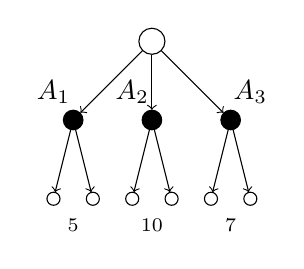
\begin{tikzpicture}
    \node[draw,circle] (root) at (2,0) {};
    \foreach \x in {1, 2, 3} {
      \node[draw,circle,fill,scale=3/4] (a\x) at (\x, -1) {};
      \draw[->] (root) -- (a\x);
      \node[draw,circle,scale=1/2] (cl\x) at (\x-.25,-2) {};
      \node[draw,circle,scale=1/2] (cr\x) at (\x+.25,-2) {};
      \draw[->] (a\x) -- (cl\x);
      \draw[->] (a\x) -- (cr\x);
    }
    \node at (0.75, -0.65) {$A_1$};
    \node at (1.75, -0.65) {$A_2$};
    \node at (3.25, -0.65) {$A_3$};
    \node[below = 1cm of a1] {\scriptsize 5};
    \node[below = 1cm of a2] {\scriptsize 10};
    \node[below = 1cm of a3] {\scriptsize 7};
  \end{tikzpicture}
  \caption{\footnotesize $v_*$ is equal to the maximum of the underbraced term in equation \ref{eq: optimalpolicyusingoptimalstatevaluefunction}, whereas $\pi_*$ is the $\argmax$. Critically, to evaluate the underbraced term for a given action, we need only perform a one step look ahead at the possible next states and rewards that follow. Imagine doing so for a particular action, labeled $A_1$, and suppose that we look at each state and reward which may follow from state $s$ after taking action $A_1$; since we have access to $v_*$ and our probability mechanics function $p$, we can evaluate each term in the summations over $s'$ and $r$. Suppose that for $A_1$ the underbraced term evaluates to $5$. We can repeat this procedure for all the actions, in this case $A_2$ and $A_3$, in each case the computation only requires a one step look ahead thanks to having access to $v_*$ and $p$. Of the three actions in this example, it happens to be that $A_2$ is the optimal action; if there were multiple maximizing actions, we could define a stochastic optimal policy that chooses between each of them with some probability.}
\end{figure}

For each state $s$, there will be one or more actions at which the maximum is obtained in the Bellman optimality equation. Any policy that assigns nonzero probability \emph{only} to these actions is an optimal policy. This is akin to a one-step search: if you have the optimal value function $v_*$, then the actions that appear best after a one-step search will be optimal actions. Put differently, any policy that is \emph{greedy} with respect to the optimal evaluation function $v_*$ is an optimal policy. The beauty of $v_*$ is that if one uses it to evaluate the short-term consequences of actions, specifically the one-step consequences, then a greedy policy is actually optimal in the long-term sense in which we are interested because $v_*$ already takes into account the reward consequences of all possible future behavior. I.e. $v_*$, the expected long run return, is turned into a quantity that is available locally and immediately available for each state. Whence, a one-step-ahead search yields the long-term optimal actions.

Let's continue with our grid-world example, building off of figure \ref{fig: valuefunctionforgammapointnine}, which we reprint below for clarity. We will use the optimal value function to learn an optimal policy.

\begin{figure}[h]
  \centering
  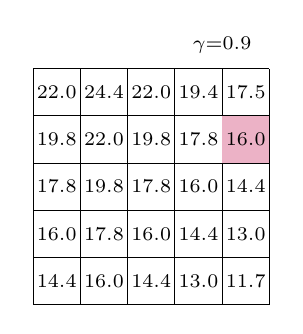
\begin{tikzpicture}[scale=0.6]
    \draw[step=1.0,black,thin] (0,0) grid (5, 5);
    % Highlight the state we're going to talk about.
    \fill[purple!30] (4,3) rectangle (5, 4);
    % Bottom row
    \node at (0.5, 0.5) {$\scriptstyle 14.4$};
    \node at (1.5, 0.5) {$\scriptstyle 16.0$};
    \node at (2.5, 0.5) {$\scriptstyle 14.4$};
    \node at (3.5, 0.5) {$\scriptstyle 13.0$};
    \node at (4.5, 0.5) {$\scriptstyle 11.7$};
    % Second to last row from bottom
    \node at (0.5, 1.5) {$\scriptstyle 16.0$};
    \node at (1.5, 1.5) {$\scriptstyle 17.8$};
    \node at (2.5, 1.5) {$\scriptstyle 16.0$};
    \node at (3.5, 1.5) {$\scriptstyle 14.4$};
    \node at (4.5, 1.5) {$\scriptstyle 13.0$};
    % Middle row
    \node at (0.5, 2.5) {$\scriptstyle 17.8$};
    \node at (1.5, 2.5) {$\scriptstyle 19.8$};
    \node at (2.5, 2.5) {$\scriptstyle 17.8$};
    \node at (3.5, 2.5) {$\scriptstyle 16.0$};
    \node at (4.5, 2.5) {$\scriptstyle 14.4$};
    % Second row from top
    \node at (0.5, 3.5) {$\scriptstyle 19.8$};
    \node at (1.5, 3.5) {$\scriptstyle 22.0$};
    \node at (2.5, 3.5) {$\scriptstyle 19.8$};
    \node at (3.5, 3.5) {$\scriptstyle 17.8$};
    \node at (4.5, 3.5) {$\scriptstyle 16.0$};
    % Top row
    \node at (0.5, 4.5) {$\scriptstyle 22.0$};
    \node at (1.5, 4.5) {$\scriptstyle 24.4$};
    \node at (2.5, 4.5) {$\scriptstyle 22.0$};
    \node at (3.5, 4.5) {$\scriptstyle 19.4$};
    \node at (4.5, 4.5) {$\scriptstyle 17.5$};
    % Gamma factor for clarity.
    \node at (4, 5.5) {$\scriptstyle \gamma = 0.9$};
  \end{tikzpicture}
  \caption{\footnotesize Consider the location or state defined by the cell that is in the second from the top row and all the way to the right; one-step look ahead considers each action and the potential next states and rewards. It's especially simple in this case because the actions leads us to deterministically pick a next state and reward. Suppose we consider the \texttt{up} action, there's no immediate reward and the next state has value $17.5$, so using $\gamma = 0.9$ and by our formula $r+\gamma v_*(s')$, this evaluates to $0 + 0.9 * 17.5 = 14$. If we take the \texttt{right} action we bump into a wall, yielding an immediate $-1$ reward and leaving us in the same state which has a value of $16$, so
$r+\gamma v_*(s')$ for this action evaluates to $-1 + 0.9 * 16 = 13.4$. The \texttt{down} action yields no immediate reward and leads us to a state with value $14.4$, and so our expression of interest evaluates to $0 + 0.9 * 14.4 = 13$. Finally, the action \texttt{left} action leads to no immediate reward but a next state value of $17.8$, and after we discount by $\gamma$ this evaluates to $0 + 0.9 * 17.8 = 16$. Of all these choices, the highest value attained is $16$, therefore, moving \texttt{left} corresponds to the optimal action in this state and \emph{must} be selected by any optimal policy. Note that for the maximizing action, the value attained is $16$ and this is indeed equal to $v_*$ for the state itself.}
\end{figure}

\begin{figure}[h]
  \centering
  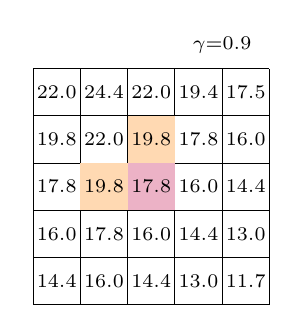
\begin{tikzpicture}[scale=0.6]
    \draw[step=1.0,black,thin] (0,0) grid (5, 5);
    % Highlight the state we're going to talk about.
    \fill[purple!30] (2,2) rectangle (3, 3);
    \fill[orange!30] (2,3) rectangle (3, 4);
    \fill[orange!30] (1,2) rectangle (2, 3);
    % Bottom row
    \node at (0.5, 0.5) {$\scriptstyle 14.4$};
    \node at (1.5, 0.5) {$\scriptstyle 16.0$};
    \node at (2.5, 0.5) {$\scriptstyle 14.4$};
    \node at (3.5, 0.5) {$\scriptstyle 13.0$};
    \node at (4.5, 0.5) {$\scriptstyle 11.7$};
    % Second to last row from bottom
    \node at (0.5, 1.5) {$\scriptstyle 16.0$};
    \node at (1.5, 1.5) {$\scriptstyle 17.8$};
    \node at (2.5, 1.5) {$\scriptstyle 16.0$};
    \node at (3.5, 1.5) {$\scriptstyle 14.4$};
    \node at (4.5, 1.5) {$\scriptstyle 13.0$};
    % Middle row
    \node at (0.5, 2.5) {$\scriptstyle 17.8$};
    \node at (1.5, 2.5) {$\scriptstyle 19.8$};
    \node at (2.5, 2.5) {$\scriptstyle 17.8$};
    \node at (3.5, 2.5) {$\scriptstyle 16.0$};
    \node at (4.5, 2.5) {$\scriptstyle 14.4$};
    % Second row from top
    \node at (0.5, 3.5) {$\scriptstyle 19.8$};
    \node at (1.5, 3.5) {$\scriptstyle 22.0$};
    \node at (2.5, 3.5) {$\scriptstyle 19.8$};
    \node at (3.5, 3.5) {$\scriptstyle 17.8$};
    \node at (4.5, 3.5) {$\scriptstyle 16.0$};
    % Top row
    \node at (0.5, 4.5) {$\scriptstyle 22.0$};
    \node at (1.5, 4.5) {$\scriptstyle 24.4$};
    \node at (2.5, 4.5) {$\scriptstyle 22.0$};
    \node at (3.5, 4.5) {$\scriptstyle 19.4$};
    \node at (4.5, 4.5) {$\scriptstyle 17.5$};
    % Gamma factor for clarity.
    \node at (4, 5.5) {$\scriptstyle \gamma = 0.9$};
  \end{tikzpicture}
  \caption{\footnotesize Let's consider a second example, this time we're considering starting from the state in the middle row and middle column. Notice that there are two actions, \texttt{up} and \texttt{left} which give the same optimal value of $0.9 * 19.8 = 17.8$. In this state, there are two different optimal actions, and an optimal policy is free to pick either (with some probability).}
\end{figure}

As a last example, consider state $A$ itself. Realize that regardless of the action we pick in state $A$, the transition dynamics dictate that we move to state $A'$ with an immediate reward of $+10$. This means that in state $A$, all actions are optimal since the transitions are equivalent. In particular $v_*(A) = 10 + \gamma * v_*(A') = 10 + 0.9 * 16 = 24.4$ which is indeed the recorded value for $v_*$ at this state.

\begin{figure}[h]
  \centering
  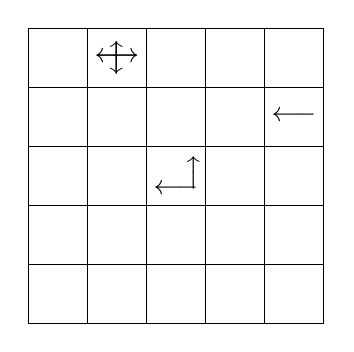
\begin{tikzpicture}[scale=0.75]
    \draw[step=1.0,black,thin] (0,0) grid (5, 5);
    \node at (1.5, 4.5) {$\longrightarrow$};
    \node at (1.5, 4.5) {$\longleftarrow$};
    \node at (1.5, 4.5) {$\big\uparrow$};
    \node at (1.5, 4.5) {$\big\downarrow$};
    \node at (4.5, 3.5) {$\longleftarrow$};
    \node at (2.5, 2.275) {$\longleftarrow$};
    \node at (2.8, 2.55) {$\big\uparrow$};
  \end{tikzpicture}
  \caption{\footnotesize We draw in a few of the optimal action(s) for various states that we've gone over above. The key idea is that we can use the Bellman optimality equation to derive an optimal policy.}
\end{figure}

Note that in the grid-world example, working out the optimal policy from $v_*$ was especially easy since each action leads us to determinstically arrive at some next state with some specified reward; so, we only had to evaluate one transition per action. But, in general the dynamics function $p$ can be stochastic, so it may not be so simple. But, as long as we have access to $p$,
we can always find the optimal action from $v_*$ by computing the right-hand side of the Bellman optimality equation for each action and finding the largest value. 

\paragraph{Using $q_*$ to determine optimal actions} With $q_*$, the agent does not even have to do a one-step-ahead search: for any state $s$ it can simply find any action that maximizes $q_*(s,a)$. The action-value function effectively caches the results of all one-step-ahead searches. Hence, at the cost of representing a function of state-action pairs instead of just states, the optimal action value function allows optimal actions to be selected without having to know anything about possible successor states and their values, i.e. without having to know anything about the environment's dynamics. In this sense, the problem of finding an optimal action-value function corresponds directly to the goal of finding an optimal policy!

\paragraph{Downsides of explicitly solving Bellman optimality equation} The approach is rarely directly useful, since it's akin to an exhaustive search which looks ahead at all possibilities, computes their probabilities of occurrence and their desireabilities in terms of expected rewards. This solution relies on three assumptions that are rarely true in practice:
\begin{enumerate}
\item We accurately know the dynamics of the environment,
\item We have enough computational resources to complete the computation of the   solution, and
\item The Markov property.
\end{enumerate}
The second limitation often means that we typically have to settle for approximate solutions.

\subsubsection{Summarizing policies, value functions, Bellman equations, and   optimality}
\paragraph{Policies}
Policies tell an agent how to behave. A deterministic policy maps each state to an action; each time a state is visited, a deterministic policy selects the associated action $\pi(s)$. Stochastic policies map each state to a distribution over all possible actions. Each time a state is visited, a stochastic policy randomly draws an action from the associated distribution with probability $\pi(a|s)$. A policy by definition depends only on the current state: it cannot depend on things like time or previous states. This is best thought of as a limitation on the state, not the agent: the state should provide the agent with all the information it needs to make a good decision.

\paragraph{Value functions} Value functions capture the future total reward under a particular policy. There are two kinds of value functions: state value functions and state-action value functions. The state value function gives hte expected return from the current state under a given policy, $v_\pi(s) \coloneqq \mathbb E_\pi \left[ G_t | S_t = s \right]$. The action-value function gives the expected return from state $s$ if the agent first selects action $a$ and follows $\pi$ after that, i.e. $q_\pi(s,a) \coloneqq \mathbb E_\pi \left[ G_t | S_t = s, A_t = a \right]$. Value functions simplify things by aggregating many possible future returns into a single number.

\paragraph{Bellman equations} The Bellman equations define a relationship between the value of a state (or state-action pair) and its successor states. The Bellman equation for the state value function gives the value of the current state as a sum over the values of all the successor states, and immediate rewards,
\[
  \color{purple} v_\pi(s) \color{black} = \sum_a \pi(a|s) \sum_{s'} \sum_r \Pr(s',r|s,a) \left[ r + \gamma   \color{purple} v_\pi(s') \color{black} \right].
\]
The Bellman equation for the action-value function gives the value of a particular state-action pair as the sum over all values of all possible next state-action pairs and rewards.
\[
  \color{purple} q_\pi(s,a) \color{black} = \sum_{s'} \sum_r \Pr(s',r|s,a) \left[ r + \gamma \sum_{a'} \pi(a'|s')  \color{purple} q_\pi(s',a') \color{black} \right].
\]
The Bellman equations can be directly solved to find the value function. These Bellman equations help us evaluate policies, but they don't achieve our ultimate goal of finding the policy that attains as much reward as possible in the long term.
\paragraph{Optimal policies} An optimal policy is one which achieves the highest possible value in every state.
\[
  v_* = v_{\pi_*}(s) = \max_\pi v_\pi(s) \hspace{15pt} \textrm{ for all } s \in \mathcal S.
  \]
There's always at least one optimal policy, but there may be more. The optimal state value function is equal to the highest possible value in every state. Every optimal policy shares the same optimal state value function. The same is true for optimal action-value functions and optimal policies.
\[
  q_* = q_{\pi_*}(s,a) = \max_\pi q_\pi(s,a) \hspace{15pt} \textrm{ for all } s \in \mathcal S \hspace{10pt} \textrm{ and } a \in \mathcal A.
\]
Like all value functions, the optimal value functions have Bellman equations
\begin{align*}
  v_{\color{purple}{\pi_*}}(s) &= \sum_a {\color{purple}\pi_*} (a|s) \sum_{s'}                                  \sum_r \Pr(s',r|s,a) \left[r + \gamma v_{\color{purple} \pi_*}(s')\right] \\
  q_{\color{purple}\pi_*}(s,a) &= \sum_{s'} \sum_r \Pr(s',r|s,a) \left[ r + \gamma \sum_{a'} {\color{purple} \pi_*}(a'|s') q_{\color{purple} \pi_*}(s',a')\right]
\end{align*}
but in this special case they do not reference any specific policy.
This amounts to replacing the policy in the Bellman equation with a \texttt{max} over all actions, since the optimal policy must always select the best available action.
\begin{align*}
  \color{orange}v_* \color{black}(s) &= {\color{orange}\max}_a \sum_{s'}                                  \sum_r \Pr(s',r|s,a) \left[r + \gamma {\color{orange}v_*}(s')\right] \\
  {\color{orange} q_*}(s,a) &= \sum_{s'} \sum_r \Pr(s',r|s,a) \left[ r + \gamma {\color{orange}\max}_{a'} {\color{purple} q_*}(s',a')\right]
\end{align*}
We can extract an optimal policy from the optimal state value function, but to do so we need the one-step dynamics of the MDP, i.e. we need our transition probabilities fully specified. We can get the optimal policy with much less work if we have the optimal action-value function: we simply select the action with the highest value in each state, i.e. $v_*(s) = \max_a q_*(s,a)$.

\subsection{Optimality and Approximation}
We've defined optimal value functions and optimal policies. Although in theory an agent that learns an optimal policy has succeeded, in practice this rarely happens. Optimal policies can only be generated with extreme computational cost. A critical aspect of the problem facing the agent is always the computational power available to it, in particular, the amount of computation it can perform in a single time step. Memory is also an important constraint, since a large amount of it is often required to built approximations of value functions, policies, and models. For tasks with small, finite state sets, we can use arrays or tables with a single entry per state (or state-action pair); this is what we call the \emph{tabular} case. Unfortunately, in many cases there are far too many states than we can store in memory. In these cases we must approximate the functions, using some sort of more compact parameterized function representation. Note that in approximating optimal behavior, there may be some states that the agent faces with such a low probability that selecting suboptimal actions has little impact on the reward the agent receives. The online nature of RL makes it possible to approximate optimal policies in ways that put more effort into learning to make good decisions for frequently encountered states, at the expense of less effort for infrequently encountered states.

\subsection{Summary of Finite MDPs}
 RL is about learning from interaction how to behave well in order to achieve a goal. The RL \emph{agent} and its \emph{environment} interact over a sequence of discrete time steps. The specification of their interface defines a particular task: the \emph{actions} are the choices made by the agent; the \emph{states} are the basis for making the choices; and the \emph{rewards} ar ethe basis for evaluating the choices. A \emph{policy} is a stochastic rule by which the agent selects actions as a function of states. The agent's objective is to maximize the amount of reward it receives over time. When RL is formulated with well-defined transition probabilities, we realize an MDP. A finite MDP has finite state, action, and reward sets. The \emph{return} is the function of future rewards that the agent seeks to maximize in expected value. There are different definitions depending on the nature of the task, i.e. for \emph{continuing} tasks we use a \emph{discounted} delayed reward whereas in \emph{episodic} tasks we use the undiscounted formulation.

A policy's \emph{value functions} assign to each state (or state-action pair) the expected return from that state (or state-action pair), given that the agent uses the policy. The \emph{optimal value functions} assign to each state (or state-action pair) the largest expected return achievable by any policy. A policy whose value functions are optimal is an \emph{optimal policy}. Any policy that is \emph{greedy} with respect to the optimal value functions must be an optimal policy. The \emph{Bellman optimality equations} are special consistency conditions that the optimal value functions must satisfy and that can, in principle, be solved for the optimal value functions, from which an optimal policy can be determined.

Even if the agent has a complete and accurate environment model, the agent is typically unable to perform enough computation per time step to fully use it. The memory available is also an important constraint, since memory may be required to build up accurate approximations of value functions, policies, and models. In most cases of interest, there are far more states than could possibly be entries in a table, and approximations must be made.

\section{Dynamic Programming}
The key idea of reinforcement learning is the use of value functions to organize and structure the search for good policies. This section is about demonstrating how dynamic programming (DP) can be used to obtain optimal policies once we have found optimal value functions, $v_*$ or $q_*$, which satisfy the Bellman optimality equations. DP algorithms are obtained by turning Bellman equations into update rules for improving approximations of the desired value functions.

\paragraph{Policy evaluation vs. control}
We often talk about two distinct tasks: policy evaluation and control. Policy evaluation is the task of determining the value function for a specific policy. Control is the task of finding a policy that obtains as much reward as possible, i.e. finding a policy which maximizes the value function. Although control is the ultimate goal of RL, the task of policy evaluation is a necessary first step, since it's hard to improve our policy if we don't have a way to assess how good it is. DP algorithms use the Bellman equations to define iterative algorithms for both policy evaluation and control. Schematically,

\begin{figure}[h]
  \centering
  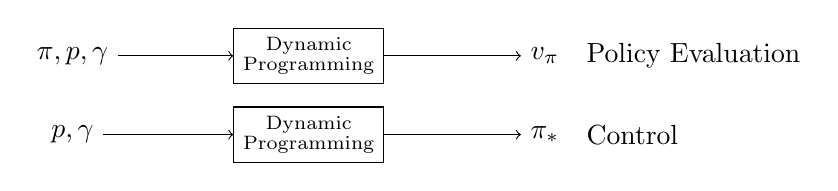
\begin{tikzpicture}
    % Policy eval
    \node (vars) at (0, 0) {$\pi, p, \gamma$};
    \node[draw,rectangle] (dp1) at (3, 0) {$\substack{\textrm{Dynamic} \\         \textrm{Programming}}$};
    \node (vpi)  at (6, 0) {$v_{\pi}$};
    \node[right = 1mm of vpi] {Policy Evaluation};
    \draw[->] (vars) -- (dp1);
    \draw[->] (dp1) -- (vpi);
    % Control
    \node (varsbottom) at (0, -1) {$p, \gamma$};
    \node[draw,rectangle] (dp2) at (3, -1) {$\substack{\textrm{Dynamic} \\         \textrm{Programming}}$};
    \node (pistar)  at (6, -1) {$\pi_*$};
    \node[right = 1mm of pistar] {Control};
    \draw[->] (varsbottom) -- (dp2);
    \draw[->] (dp2) -- (pistar);
  \end{tikzpicture}
  \caption{\footnotesize DP uses the various Bellman equations along with knowledge of $p$ to work out value functions and optimal policies. Classical DP does not involve interaction with the environment at all. It turns out that most RL algorithms can be seen as an approximation to DP programming without the model of the MDP specified?}
\end{figure}


% Recall that \emph{control} is the task of improving a policy, and that a policy % $\pi_2$ is considered as good or better than $\pi_1$ if the value under $\pi_2$ % is greater than or equal to the value under $\pi_1$ in every state; $\pi_2$ is % \emph{strictly} better if $\pi_2$ is as good or better than $\pi_1$ \emph{and} % there's at least one state in $\pi_2$ where the value under $\pi_2$ is strictly % greater than the value under $\pi_1$. The goal of the control task is to modify % a policy to produce a new one which is strictly better; we can try to improve % our policy repeatedly to obtain a sequence of better and better policies.

\subsection{Policy Evaluation (Prediction)} Let's consider how to compute the state-value function $v_\pi$ for arbitrary policy $\pi$; in the literature this is known as \emph{policy evaluation}, but we also refer to it as the \emph{prediction problem}. I.e our task is to learn a mapping $\pi \longrightarrow v_\pi$. Recall that
\begin{align}
  v_\pi(s) &\coloneqq \mathbb E_\pi \left[ G_t | S_t = s \right] \nonumber \\
           &= \mathbb E_\pi \left[ R_{t+1} + \gamma G_{t+1} | S_t = s \right] \nonumber  \\
           &= \mathbb E_\pi \left[ R_{t+1} + \gamma v_\pi(S_{t+1}) | S_t = s                           \right] \nonumber  \\
  \label{eq: framingthepredictionproblem}
           &= \sum_a \pi(a|s) \sum_{s', r} \Pr(s',r|s,a) \left[ r + \gamma v_\pi(s')\right],
\end{align}
where $\pi(a|s)$ is the probability of taking action $a$ in state $s$ under policy $\pi$, and the expectations are subscripted by $\pi$ to denote that they are conditioned on $\pi$ being followed. Recall that the Bellman equation reduces the problem of finding $v_\pi$ to a system of linear equations, one equation for each state. So, the problem of policy evaluation reduces to solving this system of linear equations, and in principle we can take a variety of methods from linear algebra to do so.

\begin{figure}[h]
  \centering
  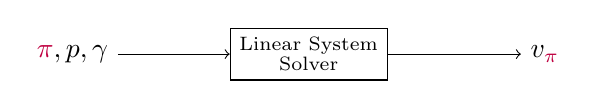
\begin{tikzpicture}
    \node (vars) at (0, 0) {$\color{purple} \pi \color{black}, p, \gamma$};
    \node[draw,rectangle] (solv) at (3, 0) {$\substack{\textrm{Linear System} \\         \textrm{Solver}}$};
    \node (vpi)  at (6, 0) {$v_{\color{purple} \pi}$};
    \draw[->] (vars) -- (solv);
    \draw[->] (solv) -- (vpi);
  \end{tikzpicture}
\end{figure}

Existence and uniqueness of $v_\pi$ are guaranteed as long as $\gamma < 1$ or eventual termination is guaranteed from all states under policy $\pi$. If the environment dynamics are completely known, then equation \ref{eq: framingthepredictionproblem} is a system of $|\mathcal S|$ simultaneous linear equations in $|\mathcal S|$ unknowns, i.e. the $v_\pi(s)$ for each $s \in \mathcal S$.

\paragraph{Iterative solutions}
In practice, iterative solution methods of DP are more suitable for general MDPs. I.e. instead of using direct solvers, lets consider a sequence of \emph{approximate} value functions, $v_0, v_1, v_2, \ldots$ which each map $\mathcal S^+$ to $\mathbb R$ (the real numbers). 
The initial approximation $v_0$ may be chosen arbitrarily, but each successive update may be obtained by using the Bellman equation for $v_\pi$ \ref{eq:   framingthepredictionproblem} as an update rule:
\begin{align}
  \label{eq: expectedupdate}
  v_{k+1}(s) &\coloneqq \mathbb E_\pi \left[R_{t+1} + \gamma v_k(S_{t+1}) | S_t     = s \right] \\
&= \sum_a \pi(a|s) \sum_{s',r} \Pr(s',r|s,a) \left[ r + \gamma v_k(s')\right] \nonumber
\end{align}
for all $s \in \mathcal S$. Realize that $v_k = v_\pi$ is a fixed-point for this update rule because the Bellman equation for $v_\pi$ assures us of equality in this case. The sequence $\{v_k\}$ can be shown in general to converge to $v_\pi$ as $k\to \infty$ under the same conditions that guarantee the existence of $v_\pi$. In practice, once $v_{k+1} = v_k$ for all states, then $v_{k} = v_\pi$ and we have found the value function.

\paragraph{Expected updates} To produce each successive approximation, $v_{k+1}$ from $v_k$, the iterative policy evaluation applies the same operation to each state $s$: it replaces the old value of $s$ with a new value obtained from the old values of the successor states of $s$, and the expected immediate rewards, along all the one-step transitions possible under the policy being evaluated. Such an operation is referred to as an \emph{expected update}. Each iteration of policy evaluation updates the value of every state once to produce a new approximate value function $v_{k+1}$.

\paragraph{In-place updates} To write the sequential compute program to implement iterative policy evaluation as given by update rule \ref{eq: expectedupdate}, you would naively have to use two arrays: one for the old values $v_k(s)$ and another for the new values $v_{k+1}(s)$. The length of these arrays would be equal to the number of states in the MDP. With these two arrays, the new values can be computed one by one from the old values without the old values being changed. It's instead easier to implement ``in place'', with each new value immediately overwriting the old one. Depending on the order in which the states are updated, sometimes new values are used instead of old ones on the right hand side of \ref{eq: expectedupdate}. This in-place algorithm is also guaranteed to converge to $v_\pi$ and is usually faster than the two-array version, since we use new data as soon as they are available.

\begin{algorithm}
  \caption{Iterative Policy Evaluation, for estimating $v_\pi$} 
  \KwInput{$\pi$, the policy to be evaluated; algorithm parameter: a small     threshold $\theta > 0$ determining accuracy of estimation}
  Initialize $V(s)$ for all $s \in \mathcal S^+$, arbitrarily except that   $V(\textrm{terminal}) = 0$. \\
\While{$\Delta \geq \theta$} {
  $\Delta \gets 0$ \\
  \For{$s \in \mathcal S$} {
    $v \gets V(s)$\\
    $V(s) \gets \sum_a \pi(a|s) \sum_{s',r} \Pr(s', r| s, a) \left[ r + \gamma       V(s')\right]$ \\
    $\Delta \gets \max\left(\Delta, |v - V(s)|\right)$ \hspace{35pt} \tcp{Track largest update to state-value function.}
  }
}
\end{algorithm}

\paragraph{Grid-world example} We consider the $4 \times 4$ gridworld shown below.
\begin{figure}[h]
  \centering
  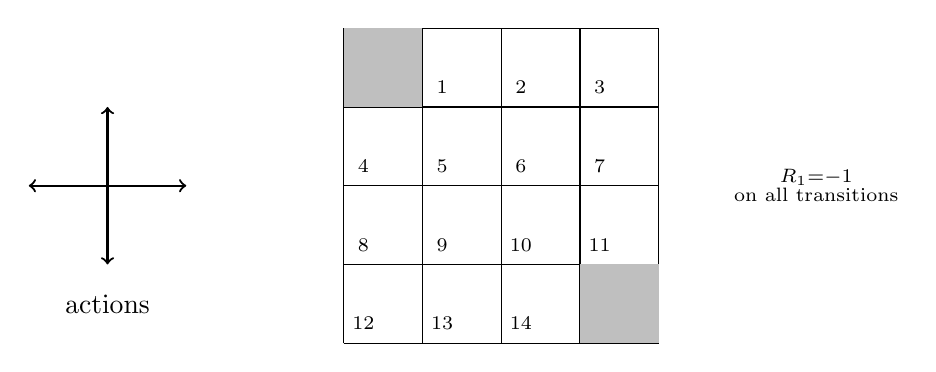
\begin{tikzpicture}
    \draw[<->,thick] (-4, 2) -- (-2, 2);
    \draw[<->,thick] (-3, 1) -- (-3, 3);
    \node at (-3, 0.5) {actions};
    \draw[step=1.0,black,thin] (0,0) grid (4, 4);
    \fill[gray!50] (0, 3) rectangle (1,4);
    \fill[gray!50] (3, 0) rectangle (4,1);
    % Top row.
    \node at (1.25, 3.25) {\scriptsize 1};
    \node at (2.25, 3.25) {\scriptsize 2};
    \node at (3.25, 3.25) {\scriptsize 3};
    % Second frop top row.
    \node at (0.25, 2.25) {\scriptsize 4};
    \node at (1.25, 2.25) {\scriptsize 5};
    \node at (2.25, 2.25) {\scriptsize 6};
    \node at (3.25, 2.25) {\scriptsize 7};
    % Second from bottom row.
    \node at (0.25, 1.25) {\scriptsize 8};
    \node at (1.25, 1.25) {\scriptsize 9};
    \node at (2.25, 1.25) {\scriptsize 10};
    \node at (3.25, 1.25) {\scriptsize 11};
    % Bottom row.
    \node at (0.25, 0.25) {\scriptsize 12};
    \node at (1.25, 0.25) {\scriptsize 13};
    \node at (2.25, 0.25) {\scriptsize 14};
    \node at (6, 2) {$\substack{R_1 = -1 \\ \textrm{on all transitions}}$};
  \end{tikzpicture}
  \caption{\footnotesize The non-terminal states are $\{1, 2, \ldots, 14\}$, and there are four possible actions in each state $\mathcal A = \{\texttt{up}, \texttt{down}, \texttt{right}, \texttt{left}\}$, which deterministically cuase the corresponding state transitions, except that actions which would take the agent off the grid in fact leave the state unchanged. In the notation of $\Pr(s',r|s,a)$ we have examples like $\Pr(6,-1|5,\texttt{right}) = 1$, or $\Pr(7, -1 | 7, \texttt{right}) = 1$, as well as $\Pr(10,r|5,\texttt{right}) = 0$ for all $r \in \mathcal R$. This is an undiscounted, episodic task. The reward is $-1$ on all transitions until the terminal state is reached, which is denoted by a gray shaded region(s); although shown in two places, it is formally one state. The expected reward function is thus $r(s,a,s') = -1$ for all states $s,s'$ and actions $a$. Suppose the agent chooses the equiprobable random policy (where all actions are equally likely). The function $v_\pi$ gives for each state the negated expected number of steps from that state until termination.}
\end{figure}

% \begin{figure}[h]
%   \centering
%   \begin{tikzpicture}[scale=2/3]
%     \node at (-2, 5) {$\substack{v_k \textrm{ for the } \\ \textrm{random % policy}}$};
%     \node at (3, 5) {$\substack{\textrm{greedy policy} \\ \textrm{w.r.t. }         % v_k}$};
%     % We first draw out all grids simultaneously, sparing values and policies % %themselves.
%     \foreach \y in {0, -1.25, ..., -6.25} {
%       \draw[step=1.0,black,thin] (-4,\y*4) grid (0, \y*4+4);      
%       \draw[step=1.0,black,thin] (1,\y*4) grid (5, \y*4+4);
%       \fill[gray!50] (1, \y*4+3) rectangle (2,\y*4+4);
%       \fill[gray!50] (4, \y*4) rectangle (5,\y*4+1);
%     }
%     % For k=0.
%     \node at (-5.5, 2) {$k=0$};
%     \foreach \x in {-3.5, ..., -0.5} {
%       \foreach \y in {0.5, ..., 3.5} {
%         \node at (\x, \y) {\scriptsize 0.0};
%       }
%     }
%     \foreach \x in {-2.5, ..., -0.5} {
%       \foreach \y in {1.5, ..., 3.5} {
%         \node at (\x + 5, \y) {$\big\uparrow$};
%         \node at (\x + 5, \y) {$\big\downarrow$};
%         \node at (\x + 5, \y) {$\longleftarrow$};
%         \node at (\x + 5, \y) {$\longrightarrow$};
%       }
%     }
%     \foreach \y in {0.5, ..., 2.5} {
%       \node at (1.5, \y) {$\big\uparrow$};
%       \node at (1.5, \y) {$\big\downarrow$};
%       \node at (1.5, \y) {$\longleftarrow$};
%       \node at (1.5, \y) {$\longrightarrow$};
%     }
%     \foreach \x in {2.5, 3.5} {
%       \node at (\x, 0.5) {$\big\uparrow$};
%       \node at (\x, 0.5) {$\big\downarrow$};
%       \node at (\x, 0.5) {$\longleftarrow$};
%       \node at (\x, 0.5) {$\longrightarrow$};
%     }
%     % For k = 1.
%     \node at (-5.5,-3) {$k=1$};
%     \node at (-5.5,-8) {$k=2$};
%     \node at (-5.5,-13) {$k=3$};
%     \node at (-5.5,-18) {$k=10$};
%     \node at (-5.5,-23) {$k=\infty$};
%   \end{tikzpicture}
% \end{figure}

\subsection{Policy Improvement}
The reason we care to compute the value function for a policy is such that we can use it to help find better policies. Suppose we've determined the value function $v_\pi$ for an \emph{arbitrary} deterministic policy $\pi$. For some state $s$, we'd like to know whether we should change the policy to deterministically choose an action $a \neq \pi(s)$. Of course, we know how good it is to follow the current policy from $s$, i.e. $v_\pi(s)$, but would it be better or worse to switch to a new policy? Consider selecting $a$ in $s$ and thereafter following the existing policy $\pi$. The value of \emph{this} way of behaving is given by
\begin{equation}
  \label{eq: takingactionathenfollowingpolicypithereafter}
  q_\pi(s,a) \coloneqq \mathbb E \left[ R_{t+1} + \gamma v_\pi(S_{t+1}) | S_t =     s, A_t = a \right] = \sum_{s',r} \Pr(s',r | s,a) \left[ r + \gamma v_\pi(s')\right].
\end{equation}
We'd like to know how this quantity compares to $v_\pi(s)$. We would intuitively expect that if it is better to select $a$ once in $s$ and thereafter follow $\pi$ relative to just following $\pi$ all the time, that we could improve our policy further still by just taking action $a$ \emph{every} time we encounter $s$. It turns out this is a special case of a general result called the \emph{policy improvement theorem}.

\subsubsection{Policy Improvement Theorem}
Let $\pi$ and $\pi'$ be any pair of deterministic policies such that for all $s \in \mathcal S$,
\begin{equation}
  \label{eq: policyimprovementthm}
  q_\pi(s, \pi'(s)) \geq v_\pi(s)
\end{equation}
then policy $\pi'$ must be as good as or better than $\pi$; i.e. it must obtain greater than or equal expected return for all states $s \in \mathcal S$: $v_{\pi'}(s) \geq v_\pi(s)$. If equation \ref{eq: policyimprovementthm} holds with \emph{strict} equality then it follows that $v_{\pi'}(s) > v_\pi(s)$. The proof behind the policy improvement theorem is easy to understand. Starting from \ref{eq: policyimprovementthm}, we continually expand out using equation \ref{eq: takingactionathenfollowingpolicypithereafter} and reapply \ref{eq:   policyimprovementthm} until we get $v_{\pi'}(s)$.

\begin{align*}
  v_\pi(s) &\leq q_\pi\left(s, \pi'(s)\right) \\
          &= \mathbb E \left[R_{t+1} + \gamma v_\pi(S_{t+1}) | S_t = s, A_t = \pi'(s)\right] &\textrm{by \ref{eq: takingactionathenfollowingpolicypithereafter}}  \\
           &= \mathbb E_{\color{purple}\pi'} \left[R_{t+1} + \gamma              v_\pi(S_{t+1}) | S_t = s \right] \\
          &\leq \mathbb E_{\pi'} \left[R_{t+1} + \gamma q_\pi(S_{t+1},             \pi'(S_{t+1})) | S_t = s\right] &\textrm{by \ref{eq: policyimprovementthm}} \\
           &= \mathbb E_{\pi'} \left[R_{t+1} + \gamma \mathbb E_{\pi'} \left[R_{t+2} + \gamma v_\pi(S_{t+2}) | S_{t+1}, A_{t+1} = \pi'(S_{t+1})\right]              | S_t = s \right] \\
           &= \mathbb E_{\pi'} \left[R_{t+1} + \gamma R_{t+2} + \gamma^2              v_\pi(S_{t+2}) | S_t = s \right] \\
           &\leq \mathbb E_{\pi'} \left[R_{t+1} + \gamma R_{t+2} + \gamma^2              R_{t+3} + \gamma^3 v_\pi(S_{t+3}) | S_t = s \right] \\
           &\hspace{5pt} \vdots \\
           &\leq \mathbb E_{\pi'} \left[R_{t+1} + \gamma R_{t+2} + \gamma^2              R_{t+3} + \gamma^3 R_{t+4} + \ldots | S_t = s \right] \\
           &= v_{\pi'}(s).
\end{align*}
So far we've seen how, given a policy and its value function, how to easily evaluate a change in the policy at a single state to a particular action. It's natural extension to consider changes at \emph{all} states and to \emph{all} possible actions, selecting at each state the action that appears to be best according to $q_\pi(s,a)$. I.e, define a \emph{greedy} policy $\pi'$ given by
\begin{equation}
  \label{eq: greedypolicy}
  \pi'(s) \coloneqq \argmax_a q_\pi(s,a) = \argmax_a \mathbb E \left[R_{t+1} + \gamma v_\pi(S_{t+1}) | S_t = s, A_t = a \right] = \argmax_a \sum_{s',r} \Pr(s',r|s,a) \left[ r + \gamma v_\pi(s')\right].
\end{equation}
\paragraph{Policy improvement}
In the even that there are multiple actions attaining a maximal value, we may break ties arbitrarily. By construction, the greedy policy meets the condition of the policy improvement theorem \ref{eq: policyimprovementthm} and so we know it's at least as good as the original policy. This process of making a new policy that improves upon an original policy, by making it greedy with respect  to the value function of the original policy, is called \emph{policy   improvement}.

\subsubsection{Why policy improvement gives us a strictly better policy} Suppose toward contradiction that the new greedy policy $\pi'$ is as good as, but not better than, the old policy $\pi$. Then, $v_\pi = v_{\pi'}$, and from equation
\ref{eq: greedypolicy} it follows that for all $s \in \mathcal S$:
\[
  v_{\pi'}(s) = \max_a \mathbb E \left[R_{t+1} + \gamma v_{\pi'}(S_{t+1}) | S_t= s | A_t = a \right] = \max_a \sum_{s',r} \Pr(s',r|s,a)\left[r + \gamma v_{\pi'}(s)\right].
\]
But, realize this is the same as the Bellman optimality equation! Therefore, $v_{\pi'}$ must be $v_*$, and both $\pi$ and $\pi'$ must be optimal policies. I.e. policy improvement therefore must give a strictly better policy except when the original policy is already optimal.

\paragraph{Stochastic optimal policies} The policy improvement theorem carries through as stated for the stochastic case where a policy $\pi$ specifies probabilities $\pi(a|s)$ for taking each action $a$ in each state $s$. If there are ties in the policy improvement steps such as \ref{eq: greedypolicy}, i.e. if there are several actions at which the maximum is achieved, then in the stochastic case we can allocate a portion of the probability of being selected in the new greedy policy to each of these maximizing actions; any portioning scheme is allowed so long as all submaximal actions are given zero probability.

\subsection{Policy Iteration (Control)}
We can iteratively improve upon our policies to obtain a sequence of monotonically improving policies and value functions.

\begin{figure}[h]
  \centering
  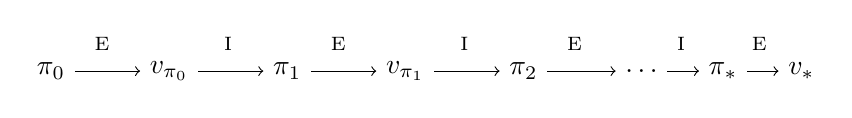
\begin{tikzpicture}
    \foreach \x in {0, 1, 2} {
      \node (p\x) at (\x * 3, 0) {$\pi_\x$};
      \node (e\x) at (\x * 3 + 0.65, 0.35) {\scriptsize E};
    }
    \foreach \x in {0, 1} {
      \node (v\x) at (\x * 3 + 1.5, 0) {$v_{\pi_\x}$};
      \draw[->] (p\x) -- (v\x);
    }
    \draw[->] (v0) -- (p1);
    \draw[->] (v1) -- (p2);
    \node at (2.25, 0.35) {\scriptsize I};
    \node at (5.25, 0.35) {\scriptsize I};
    \node (dots) at (3*2 + 1.5,  0) {$\ldots$};
    \draw[->] (p2) -- (dots);
    \node[right = 4mm of dots] (pistar) {$\pi_*$};
    \draw[->] (dots) -- (pistar);
    \node[right = 9.6mm of e2] (finali) {\scriptsize I};
    \node[right = 4mm of pistar] (vstar) {$v_*$};
    \draw[->] (pistar) -- (vstar);
    \node[right = 6mm of finali] {\scriptsize E};
  \end{tikzpicture}
  \caption{\footnotesize In this figure, $\overset{\textrm{E}}{\longrightarrow}$ denotes a policy \emph{evaluation} and $\overset{\textrm{I}}{\longrightarrow}$ denotes a policy \emph{improvement}. Each policy is deterministic, and is guaranteed to be strictly better than the last, unless it's already optimal. Because a finite MDP has only a finite number of deterministic policies, this process must converge to an optimal policy and optimal value function in a finite number of iterations.}
\end{figure}

This way of finding an optimal policy is known as \emph{policy iteration}. We provide a complete sequence of instructions in algorithm \ref{alg: policyimprovement}.
Notice that in the step of Policy Evaluation, that we are using the value functions learned from our previous policy; this typically results in a large increase in the speed of convergence of our algorithm, presumably because the value function is changing slowly from one policy to the next.

\begin{algorithm}[h]
  \SetKwRepeat{Do}{do}{while}
  \KwInput{$\theta$, a small positive number determining the accuracy of         estimation.}
  Initialize $V(s) \in \mathbb R$ and $\pi(s) \in \mathcal A(s)$ arbitrarily for   all $s \in \mathcal S$ \tcp{Initialization.}
\tcp{Policy Evaluation (make $v$ reflect $\pi$).}
\Do{$\Delta \geq \theta$}{
  $\Delta \gets 0$ \\
  \For{$s \in \mathcal S$} {
    $v \gets V(s)$ \\
    $V(s) \gets \sum_{s',r} \Pr(s',r|s, \pi(s))\left[r + \gamma V(s')\right]$ \\
    $\Delta \gets \max\{\Delta, |v - V(s)|\}$
  }
}
\tcp{Policy improvement (make $\pi$ greedy).}
\texttt{policy\_stable} $\gets$ \texttt{true} \\
\For{$s \in \mathcal S$} {
  \texttt{old\_action} $\gets \pi(s)$ \\
  $\pi(s) \gets \argmax_a \sum_{s',r} \Pr(s',r|s,a) \left[r + \gamma     V(s')\right]$ \\
\lIf{\texttt{old\_action} $\neq \pi(s)$}{
  \texttt{policy\_stable} $\gets \texttt{false}$
}
}
\lIf{\texttt{policy\_stable}} {
  \Return{$V \approx v_*$ and $\pi \approx \pi_*$}
} \lElse{
  Evaluate policy, going back to second step in our algorithm.
}
\caption{\footnotesize Policy Iteration (using iterative policy evaluation) for estimating $\pi \approx \pi_*$. Note that this algorithm can oscillate between two equally good policies, and so in practice we should keep track of whether our value function is changing (i.e. still improving) in addition to checking for \texttt{policy\_stable}.}
\label{alg: policyimprovement}
\end{algorithm}

\begin{figure}[h]
  \centering
  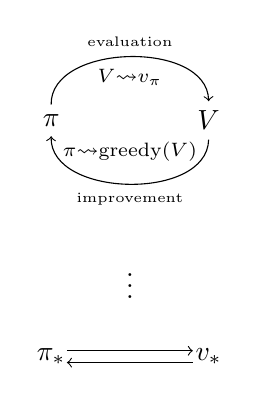
\begin{tikzpicture}
    \node (pi) at (-1, 0) {$\pi$};
    \node (v)  at ( 1, 0) {$V$};
    \path[->] (pi) edge[bend left = 90] (v);
    \path[->] (v)  edge[bend left = 90] (pi);
    \node at (0, 1) {\tiny evaluation};
    \node at (0, 0.55) {$\scriptstyle V \leadsto v_\pi$};
    \node at (0, -0.4) {$\scriptstyle \pi \leadsto \textrm{greedy}(V)$};
    \node at (0, -1) {\tiny improvement};
    \node at (0, -2) {$\vdots$};
    \node (pistar) at (-1, -3) {$\pi_*$};
    \node (pistar) at (1, -3) {$v_*$};
    \draw[->] (-.8, -2.925) -- (.8, -2.925);
    \draw[<-] (-.8, -3.075) -- (.8, -3.075);
  \end{tikzpicture}
  \caption{\footnotesize We use the term \emph{generalized policy iteration} (GPI) to refer to the general idea of letting policy evaluation and policy improvement processes interact, independent of the granularity and other details of the two processes. Almost all RL learning methods can be described as GPI: i.e. all have identifiable policies and value functions, with the policy always being improved with respect to the value function and the value function always being driven toward the value function for the policy, as suggested in our diagram. If both the evaluation process and improvement process stabilize, then the value function and policy must be optimal: the value function only stabilizes when it is consistent with the current policy, and the policy stabilizes only when it is greedy with respect to the current value function. Thus, both processes stabilize only when a policy has been found that is greedy with respect to its own evaluation function. This implies the Bellman optimality equation holds and thus that the policy and value function are optimal!}
\end{figure}

\begin{figure}[h]
  \centering
  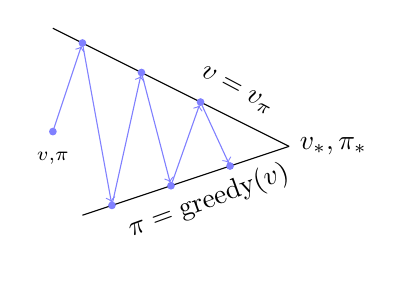
\begin{tikzpicture}[scale=3/4]
    \draw (-4, 2) -- (0, 0) node[above left = 3mm, rotate = -28] {$v = v_\pi$};  % y = -1/2x
    \draw (-3.5,-1.16666) -- (0, 0) node[below left, rotate=20] {$\pi =       \textrm{greedy}(v)$}; % y= 1/3*x
    \node at (0.75, 0) {$v_*, \pi_*$};
    \node[draw,circle,fill,scale=1/4,blue!50] (init) at (-4, 0.25) {};
    \node[below = 1mm of init] {$\scriptstyle v,\pi$};
    \node[draw,circle,fill,scale=1/4,blue!50] (one)  at (-3.5, 1.75) {};
    \node[draw,circle,fill,scale=1/4,blue!50] (two)  at (-3, -1) {};
    \node[draw,circle,fill,scale=1/4,blue!50] (three)at (-2.5, 1.25) {};
    \node[draw,circle,fill,scale=1/4,blue!50] (four) at (-2, -2/3) {};
    \node[draw,circle,fill,scale=1/4,blue!50] (five) at (-1.5, 0.75) {};
    \node[draw,circle,fill,scale=1/4,blue!50] (six)  at (-1, -1/3) {};
    \draw[->,blue!50] (init) -- (one);
    \draw[->,blue!50] (one) -- (two);
    \draw[->,blue!50] (two) -- (three);
    \draw[->,blue!50] (three) -- (four);
    \draw[->,blue!50] (four) --(five);
    \draw[->,blue!50] (five) -- (six);
  \end{tikzpicture}
  \caption{\footnotesize We can think of the nteraction between the evaluation and improvement processes in GPI in terms of two constraints or goals -- for example as two lines in two-dimensional space as suggested by the diagram. Although the real geometry is much more complicated, the diagram suggests what happens in the real case. Each process drives the value function or policy toward one of the lines representing a solution to one of the two goals. The goals \emph{interact} because the lines are not orthogonal: driving directly toward one goal causes some movement away from the other goal; inevitably, however, the joint process is brought closer to the overall goal of optimality. The arrows in the diagram correspond to the behavior of policy iteration in that each takes the system all the way to achieving one of the two goals completely. In GPI, one could also take smaller, incomplete steps toward each goal. In either case, the two processes together achieve the overall goal of optimality even though neither is attempting to achieve it directly!}
\end{figure}
\subsection{Value Iteration}
A downside to policy iteration is that each of its iterations involves policy evaluation, which may itself be an iterative computation involving multiple sweeps through the state set. If policy evaluation is done iteratively, it is only in the limit that we get convergence to $v_\pi$. The policy evaluation step of policy iteration can be truncated in several ways without losing the convergence guarantees of policy iteration! One important case is when the algorithm is stopped after just one sweep (or one update of each state). This algorithm is known as \emph{value iteration}. It can be written as a particularly simple update operation that combines the policy improvement and truncated policy evaluation steps:

\begin{equation}
  v_{k+1} \coloneqq \max_a \mathbb E \left[ R_{t+1} + \gamma v_k(S_{t+1}) | S_t = s , A_t = a \right] = \max_a \sum_{s',r} \Pr(s',r|s,a) \left[ r + \gamma v_k(s')\right],
\end{equation}

for all $s \in \mathcal S$. For any arbitrary $v_0$, the sequence $\{v_k\}$ can be shown to converge to $v_*$ under the same conditions that guarantee the existence of $v_*$. Realize that value iteration is obtained simply by turning the Bellman optimality equation into an update rule. Also, note that the value iteration update is identical to the policy evaluation update \ref{eq:     expectedupdate} except it requires the maximum to be taken over all actions.

\paragraph{How does value iteration terminate?} Like policy evaluation, value iteration formally requires an infinite number of iterations to converge exactly to $v_*$. In practice, we stop once the value function changes by only a small amount in a sweep.

\begin{algorithm}[h]
  \SetKwRepeat{Do}{do}{while}
  \KwInput{A small threshold $\theta > 0$ determining accuracy of estimation}
  Initialize $V(s)$, for all $s \in \mathcal S^+$, arbitrarily except that   $V(\textrm{terminal}) = 0$. \\
\Do{$\Delta < \theta$} {
  $\Delta \gets 0$ \\
  \For{$s \in \mathcal S$} {
    $v \gets V(s)$ \\
    \tcp{\footnotesize In the next step, we don't refer to any policy, hence name value iteration}
    $V(s) \gets \max_a \sum_{s',r} \Pr(s',r|s,a)\left[r+\gamma V(s')\right]$ \\    $\Delta \gets \max\{\Delta, |v-V(s)|\}$
  }
}
Output a deterministic policy, $\pi \approx \pi_*$, such that
\[
  \pi(s) = \argmax_a \sum_{s',r} \Pr(s',r|s,a) \left[ r + \gamma V(s')\right].
\]
\caption{Value iteration, for estimating $\pi \approx \pi_*$}
\end{algorithm}

Value iteration effectively combines, each each of its sweeps, one sweep of policy evaluation and one sweep of policy improvement.

\paragraph{Asynchronous DP}
Methods that perform systematic sweeps like this are called synchronous; this can be problematic if the state space is large since the sweeps can take a long time. Asynchronous DP is a family of methods in which we update the states in any order; in fact, multiple updates may be performed to a single state before another state is updated once. In order to guarantee convergence, asynchronous algorithms must update the values of all states.

\subsection{Generalized Policy Iteration}
Policy iteration consists of two simultaneous, interacting processes: one making the value function consistent with the current policy (policy evaluation), and the other making the policy greedy with respect to the current value function (policy improvement). In policy iteration, these two processes alternate, but this isn't necessary as we saw in value iteration only a single iteration of policy evaluation is performed in between each policy improvement.  As long as both processes continue to update all states, the ultimate result is typically the same - convergence to the optimal value function and an optimal policy.

\paragraph{Evaluation and Improvement as both competing and cooperating processes}
The evaluation and improvement processes in GPI are both competing and cooperating processes. They compete in the sense that making the policy greedy with respect to the value function typically makes the value function incorrect for the changed policy, and making the value function consistent with the policy typically causes the policy no longer to be greedy. In the long run, however, these two processes interact to find a single joint solution: the optimal value function and an optimal policy.

\subsection{Efficiency of Dynamic Programming}
For very large problems, DP is not practical. But, compared with other methods for solving MDPs, DP methods are actually quite efficient. The worst case work required by DP methods to find an optimal policy is polynomial in the number of states and actions. If $n$ and $k$ denote the number of states and actions, this means that a DP method takes a number of computational operations that is less than some polynomial function of $n$ and $k$. Note that we find an optimal policy in polynomial time even tohugh the total number of (deterministic) policies is $k^n$; in this sense, DP is exponentially faster than any direct search in policy space could be. DP is sometimes thought to be of limited applicability because of the \emph{curse of dimensionality}, the fact that the number of states often grows exponentially with the number of state variables. Although it's true that large state sets create difficulties, these are inherent difficulties in the problem not of DP as a solution method. DP is in fact comparatively better suited to handling large state spaces than competing methods such as direct search and linear programming.

\subsubsection{Monte Carlo sampling as an alternative method for learning a     value function}
The value of each state can be treated as a totally independent estimation problem. First, recall that the value of a state is given by the expected reward starting from that state when acting under a particular policy, i.e.
\[
  v_\pi(s) \coloneqq \mathbb E_\pi\left[G_t | S_t = s \right].
\]
First, let's gather a large number of returns under $\pi$ and then take their average for each state; this method is called the Monte Carlo method. However, if we do it this way we may need a large number of returns from each state. To see this, realize that each return depends on many random actions, selected by $\pi$, as well as many random state transitions due to the dynamics of the MDP. We could be dealing with a lot of randomness here, and so each return might be very different than the true state value. So, we may need to average many returns before the estimate converges, and we have to do this for every single state. 

\paragraph{DP bootstraps value estimates from successor states to improve current value estimate} 
The key insight to DP is that we don't have to treat the evaluation of each state as a separate problem: we can use the other value estimates that we've worked hard to compute. The process of using the value estimates of successor states to improve our current value estimate is known as \emph{bootstrapping}. This can be much more efficient than a Monte-Carlo method which estimates each value independently.

\subsubsection{Brute-force search as an alternative method for finding an   optimal policy}
Here, we simply evaluate every possible deterministic policy one at a time. We then select the one with the highest value. Since there are a finite number of deterministic policies, there always exists an optimal deterministic policy. So, brute-force search will find the answer eventually. However, the number of deterministic policies can be huge. Because a deterministic policy consists of one action choice per state, the total number of deterministic policies is exponential in the number of states; i.e. there are $|\mathcal S|$ states, and for each we have to consider from $|\mathcal A|$ different actions, this leads to multiplying $|\mathcal A|$ by itself $|\mathcal S|$ times: $|\mathcal A|^{|\mathcal S|}$. On the other hand, the policy improvement theorem guarantees that policy iteration will find a sequence of better and better policies: this is a significant improvement over exhaustively searching each and every policy. 

\subsection{Summary}
Policy evaluation is the task of determining the state-value function $v_\pi$ for a particular policy $\pi$. Iterative policy evaluation takes the Bellman equation for $v_\pi$,
\[
  v_\pi(s) = \sum_a \pi(a|s) \sum_{s'} \sum_r \Pr(s',r|s,a)\left[r + \gamma v_\pi(s')\right]
\]
and turns it into an update rule, producing better and better approximations for $v_\pi$:
\[
  v_{k+1} \gets \sum_a \pi(a|s) \sum_{s'} \sum_r \Pr(s',r|s,a) \left[ r + \gamma v_k(s')\right].
\]
Control refers to the task of improving a policy. The policy improvement theorem tells us how to construct a better policy from a given policy:
\[
  \pi'(s) \coloneqq \argmax_a \sum_{s'} \sum_r \Pr(s',r|s,a) \left[ r + \gamma v_\pi(s')\right].
\]
The new policy $\pi'$ is produced by ``greedifying'' with respect to current values. We are guaranteed to yield a better policy unless what we started with was already optimal. The DP algorithm for control is built upon the policy improvement theorem; this algorithm is called policy iteration. It consists of two steps: policy evaluation and improvement. In policy evaluation, we find the value function for the current policy. Policy improvement or ``greedification'' makes the policy greedy with respect to the current value functions. These steps are repeated over and over until the policy doesn't change, in which case we are guaranteed to have found an optimal policy. We discussed the framework of generalized policy iteration, in which the evaluation and improvement steps need not be run to completion; one example is the value iteration algorithm. Generalized policy iteration also includes asynchronous methods, which can more efficiently propagate value information This can be particularly helpful if the state space is very large.

\section{Sample-based Learning Methods}
Sample-based learned methods mean that we learn solely from trial and error, i.e. from experience. All agents can learn how the world works on their own, and we do not need to specify a model of the world any longer. If we do have a model, we can still use it by simulating experience from it. Sample-based learning algorithms are based on value functions and ideas from DP, including one of the most fundamental algorithms in RL called temporal difference learning. We first start with methods to learn value functions for prediction, then we'll see how we can learn action values for control, and finally we'll talk about planning with our learned model. We will discuss Monte-Carlo methods, and how TD methods can be used for prediction and control. We'll also see how TD control methods like SARSA and Q-learning are connected to generalized policy iteration and Bellman operators. Along the way, we'll discuss expiration, which is critical when learning from trial and error interaction. Further, we'll learn about off-policy learning, which is essential when learning from experience.

\subsection{Monte Carlo methods}
Here, we do not assumpe complete knowledge of the environment; instead we only require \emph{experience} -- sample sequences of states, actions, and rewards from actual or simulated interaction with an environment. Learning from \emph{actual} experience is striking because it requires no knowledge of the environment's dynamics, and yet an optimal policy can still be obtained. Learning from \emph{simulated} experiences is powerful, and although a model is required it need only generate sample transitions as opposed to complete probability distributions of all possible transitions that is required for DP. Monte Carlo methods are a way of solving RL problems by averaging sample (complete) returns; we focus only on episodic tasks such that returns are well defined. In particular, Monte Carlo methods sample and average \emph{returns} for each state-action pair, and average \emph{rewards} for each action. Whereas we previously computed value functions from knowledge of the MDP, here we \emph{learn} value functions from sample returns with the MDP. Value functions and corresponding policies still interact to attain optimality in the same way (GPI).

\subsubsection{Monte Carlo Prediction}
Recall that the value of a state is the expected return -- expected cumulative future discounted reward--starting from that state. An obvious way to estimate it from experience is by averaging returns observed after visits to that state; as more returns are observed, weak law of large numbers guarantees the sample average converges in probability to the population mean. This idea underlies all Monte Carlo methods. In particular, suppose we wish to estimate $v_\pi(s)$, the value of a state $s$ under policy $\pi$, given a set of episodes obtained by following $\pi$ and passing through $s$. Each occurrence of state $s$ in an episode is called a \emph{visit} to $s$. Note that $s$ may be visited multiple times in the same episode; let us define the first time it is visited as the \emph{first visit} to $s$. The \emph{first-visit MC method} estimates $v_\pi(s)$ as the average of the returns following first visits to $s$, whereas the \emph{every visit MC method} averages the returns following all visits to $s$.
\begin{algorithm}[h]
  \caption{First-visit MC prediction, for estimating $V \approx v_\pi$}
  \KwInput{A policy $\pi$ to be evaluated}
  \tcp{Initialization.}
  $V(s) \in \mathbb R$ arbitrarily, for all $s \in \mathcal S$ \\
  $\texttt{Returns}(s) \gets$ an empty list, for all $s \in \mathcal S$ \\
  \While{True} {
    Generate an episode following $\pi$: $S_0, A_0, R_1, S_1, A_1, R_2,     \ldots,S_{T-1}, A_{T-1}, R_T$ \\
    $G\gets 0$ \\
    \For{$t = T-1, T-2, \ldots, 0$} {
      $G \gets \gamma G + R_{t+1}$ \\
      \If{$S_t$ not in $S_0, S_1, \ldots, S_{t-1}$} {
        Append $G$ to $\texttt{Returns}(S_t)$ \\
        $V(S_t) \gets \texttt{average}(\texttt{Returns}(S_t))$
      }
    }
  }
\end{algorithm}
Both first-visit and every-visit MC converge to $v_\pi(s)$ as the number of visits (or first visits) to $s$ goes to $\infty$. It's particularly easy to see in the case of first-visit MC: each return is an independent, identically distributed estimate of $v_\pi(s)$ with finite variance; by weak law of large numbers the sequence of averages of these estimates converges to their true expected value; each average itself is an unbiased estimate and the standard deviation of its error decreases like $\frac{1}{\sqrt n}$, where $n$ is the number of returns averaged.

\paragraph{Blackjack Example} The goal is to obtain cards the sum of whose numerical values is as great as possible without exceeding 21. All face cards count as 10, an ace can count as either 1 or 11. We consider a game where we only play against the dealer. The game starts with two cards dealt to both dealer and player. \emph{One of the dealer's cards is face up and the other is face down.} If the player has 21 immediately (an ace and a 10-card), then it is called a natural and he/she wins unless the dealer also has a natural in which case we pronounce a draw. If the player doesn't have a natural, he/she can either request an additional card (hit), stop requesting cards (stick), or go bust (if the value of cards exceeds 21). If he/she goes bust, the agent loses. If the agent sticks, it becomes the dealer's turn. The dealer hits or sticks according to a fixed strategy: stick on any sum 17 or greater, and hits otherwise. If the dealer goes bust the agent wins; otherwise, the outcome is determined by whosever final sum is closer to 21. This problem is naturally formulated as an episodic MDP, where each game is an episode. Rewards of +1, -1, and 0 are given for winning, losing, and drawing respectively; all rewards within a game are zero, and we don't discount. Whence, the terminal rewards are also the returns. The agent's \emph{actions} are to hit or to stick. The states depend on the player's cards and the dealer's showing card. We assume the cards are dealt from an infinite deck (i.e. with replacement) so that there is no advantage to keeping track of which cards are already dealt. If the player holds an ace that he/she could count as 11 without going bust, then the ace is said to be \emph{useable}. In this case, it is always counted as 11, because counting it as a 1 would make the sum 11 or less, in which case there is no decision to be made because obviously the player should always hit (since in this case a hit is impossible to cause a bust, since the max valued card is 10 ignoring aces which can be treated as ones). Thus, the player makes their decision based on three variables: their current sum (12-21), the dealer's one showing card (ace-10), and whether or not he/she holds a useable ace. This makes for a total of 200 states. We consider the policy that sticks if the player's sum is 20 or 21, and otherwise hits. To find the state-value function for this policy by a Monte Carlo approach, we simulate many blackjack games using the policy and average the returns following each state.

\paragraph{Comparing why DP not suitable for task of blackjack} Although we have complete knowledge of the environment in the blackjack task, it wouldn't be easy to apply DP methods to compute the value function. DP methods requrie the distribution of next events -- in particular, they require the environments dynamics as given by the four-argument function $\Pr(s', r | s, a)$ -- and it is not easy to determine this for blackjack. E.g. suppose the player's sum is 14 and they choose to stick. What is the probability of the agent terminating with a reward of $+1$ as a function of the dealer's showing card? All of the probabilities must be computed \emph{before} DP can be applied, and these computations are complex and error-prone for this example. In contrast, generating the sample games required by MC methods is easy, and this is the case surprisingly often.

\paragraph{Backup diagrams and Monte Carlo algorithms} The general idea of a backup diagram is to show at the top the root node to be updated and to show below all the transitions and leaf nodes whose rewards and estimated values contribute to the update. For Monte Carlo evaluation of $v_\pi$, the root is a state node, and below it is an entire trajectory of transitions along a particular single episode, ending at the terminal state.

\begin{figure}[h]
  \centering
  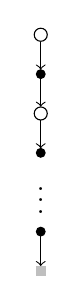
\begin{tikzpicture}[scale=1/2]
    \node[draw,circle,scale = 1/2] (root) at (0, 0) {};
    \node[draw,circle,fill,scale=1/3] (a1) at (0, -1) {};
    \node[draw,circle,scale = 1/2] (s1) at (0, -2) {};
    \node[draw,circle,fill,scale=1/3] (a2) at (0, -3) {};
    \node (dots) at (0,-4) {$\vdots$};
    \node[draw,circle,fill,scale=1/3] (an) at (0,-5) {};
    \node[draw,rectangle,fill,gray!50,scale=1/2] (sn) at (0,-6) {};
    \draw[->] (root) -- (a1);
    \draw[->] (a1) -- (s1);
    \draw[->] (s1) -- (a2);
    \draw[->] (an) -- (sn);
  \end{tikzpicture}
\end{figure}

Whereas the DP diagram shows all possible transitions, the Monte Carlo diagram shows only those sampled on the one episode. Whereas the DP diagram includes only one-step transitions, the Monte Carlo diagram goes all the way to the end of the episode. These differences in the diagrams accurately reflect the fundamental differences between the algorithms.

\paragraph{Monte Carlo methods imply estimates for each state are independent} The estimate for one state does not depend or build upon the estimate of any other state, as in the sense of DP. In other words, Monte Carlo methods do not \emph{bootstrap} as defined previously.

\paragraph{Computational expense of estimating the value of a single state is independent of the number of states} This can make Monte Carlo methods particularly attractice when one requires the value of only one or a subset of states. One can generate many sample episodes starting from the states of interest, averaging returns from only these states, ignoring all others. This is a third advantage of Monte Carlo methods can have over DP method, after the ability to learn from (simulated) experience.

\subsubsection{Monte Carlo Estimation of Action Values}
If a model is not available, then it is particularly useful to estimate \emph{action} values (the value of state-action pairs) rather than \emph{state} values. With a model, state values alone are sufficient to determine a policy: one simply looks one step ahead and chooses whichever action leads to the best combination of reward and next state. Without a model, however, state values alone are not sufficient: one must explicitly estimate the value of each action in order for the values to be useful in suggesting a policy. Thus, a primary goal for Monte Carlo methods is to estimate $q_*$. To achieve this, we consider the policy evaluation problem for action values.

\paragraph{Policy evaluation problem for action values} The problem is to estimate $q_\pi(s,a)$, the expected return when starting in state $s$, taking action $a$, and thereafter following policy $\pi$. The Monte Carlo methods for this are essentially the same as just presented for state values, except now we talk about visits to a state-action pair rather than to a state. A state-action pair $s,a$ is said to be visited in an episode if ever the state $s$ is visited and action $a$ is taken in it. The every-visit MC method estimates the value of a state-action pair as the average of the returns that have followed all the visits to it, whereas the first-visit MC method averages the returns following the first time in each episode that the state was visited and the action was selected. These method both converge to the true expected values as the number of visits to each state-action pair approaches infinity.

\paragraph{The general problem of maintaining exploration} There is a complication in that many state-action pairs may never be visited. If $\pi$ is a deterministic policy, then in following $\pi$ one will observe returns only for one of the actions from each state. With no returns to average, the Monte Carlo estimates of the other actions will not improve with experience. This is problematic because the purpose of learning action values is to help in choosing among the actions available in each state. To compare alternatives, we need to estimate the value of \emph{all} the actions from each state, not just the one we currently favor. This is the problem of \emph{maintaining exploration}.

\paragraph{The method of exploring starts}
For policy evaluation to work for action values, we must assure continual exploration. One way to do this is by specifying that the episodes \emph{start in a state-action pair}, and that every pair has a nonzero probability of being selected as the start. This guarantees that all state-action pairs will be visited an infinite number of times in the limit of an infinite number of episodes. This strategy is known as \emph{exploring starts}. Although this method is sometimes useful, it cannot be relied upon in general, particularly when learning directly from actual interaction with an environment. In that case, the starting conditions are unlikely to be so helpful. The most common alternative approach to assuring that all state-action pairs are encountered is to consider only policies that are stochastic with a nonzero probability of selecting all actions in each state.
\subsubsection{Monte Carlo Control}
We can now consider how MC estimation can be used in control, i.e. to approximate better policies. The overall idea is to proceed according to the idea of generalized policy iteration; we will maintain both an approximate policy and an approximate value function. The value function is repeatedly altered to more closely approximate the value function for the current policy, and the policy is repeatedly improved with respect to the current value function. Although the two changes work against each other to some extent, as each creates a moving target for the other, they cause both policy and value function to approach optimality.

\paragraph{Monte Carlo version of classical policy iteration} In this method, we perform alternating complete steps of policy evaluation and policy improvement, beginning with an arbitrary policy $\pi_0$ and ending with the optimal policy and optimal action-value function.
\begin{figure}[h]
  \centering
  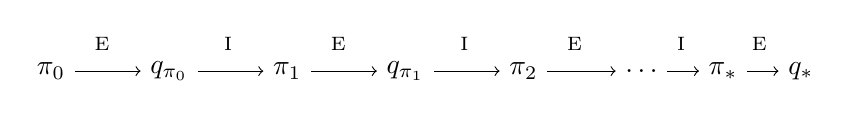
\begin{tikzpicture}
    \foreach \x in {0, 1, 2} {
      \node (p\x) at (\x * 3, 0) {$\pi_\x$};
      \node (e\x) at (\x * 3 + 0.65, 0.35) {\scriptsize E};
    }
    \foreach \x in {0, 1} {
      \node (v\x) at (\x * 3 + 1.5, 0) {$q_{\pi_\x}$};
      \draw[->] (p\x) -- (v\x);
    }
    \draw[->] (v0) -- (p1);
    \draw[->] (v1) -- (p2);
    \node at (2.25, 0.35) {\scriptsize I};
    \node at (5.25, 0.35) {\scriptsize I};
    \node (dots) at (3*2 + 1.5,  0) {$\ldots$};
    \draw[->] (p2) -- (dots);
    \node[right = 4mm of dots] (pistar) {$\pi_*$};
    \draw[->] (dots) -- (pistar);
    \node[right = 9.6mm of e2] (finali) {\scriptsize I};
    \node[right = 4mm of pistar] (vstar) {$q_*$};
    \draw[->] (pistar) -- (vstar);
    \node[right = 6mm of finali] {\scriptsize E};
  \end{tikzpicture}
  \caption{\footnotesize In this figure, $\overset{\textrm{E}}{\longrightarrow}$ denotes a complete policy \emph{evaluation} and $\overset{\textrm{I}}{\longrightarrow}$ denotes a complete policy \emph{improvement}.}
\end{figure}

For the moment, we assume that we do indeed observe an infinite number of episodes and additionally that the episodes are generated with exploring starts. Under these assumptions the Monte Carlo methods will compute each $q_{\pi_k}$ exactly, for arbitrary $\pi_k$.

\paragraph{Policy Improvement} Policy improvement is done by making the policy greedy with respect to the current value function. In this case we have an \emph{action}-value function, and therefore no model is needed to construct the greedy policy. For any action-value function $q$, the corresponding greedy policy is the one that, for each $s \in \mathcal S$, deterministically chooses an action with maximal action-value, i.e.
\[
  \pi(s) \coloneqq \argmax_a q(s,a).
\]
Policy improvement then can be done by constructing each $\pi_{k+1}$ as the greedy policy with respect to $q_{\pi_k}$.
The policy improvement theorem then applies to $\pi_k$ and $\pi_{k+1}$ because for all $s \in \mathcal S$:
\[
  q_{\pi_k}(s, \pi_{k+1}(s)) = q_{\pi_k}(s, \argmax_a q_{\pi_k}(s,a)) = \max_a q_{\pi_k} (s,a) \geq q_{\pi_k}(s, \pi_k(s)) \geq v_{\pi_k}(s).
\]
Whence our policy improvement assures us that eacy $\pi_{k+1}$ is uniformly better than $\pi_k$, or just as good as it, in which case they are both optimal policies. This ensures that the overall process converges to the optimal policy and optimal value function; in this way Monte Carlo methods can be used to find optimal policies given only sample episodes and no other knowledge of the environment's dynamics.

\paragraph{Removing the assumption that policy evaluation operates on an infinite number of episodes} There are two approaches. One is to hold firm to the idea of approximating $q_{\pi_k}$ in each policy evaluation; measurements and assumptions are made to obtain bounds on the magnitude and probability of error in the estimates, and then sufficient steps are taken during each policy evaluation to ensure that these bounds are sufficiently small. Although this approach can guarantee convergence, it doesn't do so fast enough. The second approach is to give up trying to complete policy evaluation before returning to policy improvement; on each evaluation step we move the value function \emph{toward} $q_{\pi_k}$, but we don't expect to get close except over many steps.\footnote{One extreme form of this idea is value iteration, in which only one iteration of iterative policy evaluation is performed before each step of policy improvement. The in-place version of value iteration is even more extreme in that we alternate between improvement and evaluation steps for single states.} For Monte Carlo policy iteration it is natural to alternate between evaluation and improvement on an episode-by-episode basis. After each episode, the observed returns are used for policy evaluation, and then the policy is improved at all the states \emph{visited} in the episode.

\begin{algorithm}[h]
  \caption{Monte Carlo Exploring Starts, for estimating $\pi \approx \pi_*$}
  \tcp{Initialize.}
  $\pi(s) \in \mathcal A(s)$ (arbitrarily), for all $s \in \mathcal S$ \\
  $Q(s,a) \in \mathbb R$ (arbitrarily), for all $s in \mathcal S, a \in \mathcal   A(s)$ \\
  $\texttt{Returns}(s,a) \gets$ empty list, for all $s in \mathcal S, a \in   \mathcal   A(s)$ \\
\For{each episode (without termination)} {
  Choose $S_0 \in \mathcal S$, $A_0 \in \mathcal A(S_0)$ randomly such that all   pairs have probability $>0$. \\
  Generate an episode from $S_0, A_0$ following $\pi$: $S_0, A_0, R_1, \ldots,   S_{T-1}, A_{T-1}, R_T$.\\
  $G \gets 0$. \\
  \For{each step of the episode $t = T-1, T-2, \ldots, 0$} {
    $G \gets \gamma G + R_{t+1}$ \\
    \If{$S_t, A_t$ does not appear in $S_0, A_0, S_1, A_1, \ldots, S_{t-1},             A_{t-1}$} {
Append $G$ to $\texttt{Returns}(S_t, A_t)$ \\
$Q(S_t, A_t) \gets \texttt{average}(\texttt{Returns}(S_t, A_t))$ \\
$\pi(S_t) \gets \argmax_a Q(S_t, a)$
    }
  }
}
\label{alg: montecarloes}
\end{algorithm}
Note that the pseudocode in algorithm \ref{alg: montecarloes} is inefficient because it maintains a listing of all returns for each state-action pair and repeatedly calculates their mean; it would be more efficient to maintain just the running average and a count (for each state-action pair) and update them incrementally.

\paragraph{Convergence of Monte Carlo with Exploring Starts}
Suppose toward contradiction that our algorithm converges to a suboptimal policy. Realize that the value function would eventually converge to the value function for that policy, and that in turn would cause the policy to change. Stability is achieved only when both the policy and the value function are optimal.

\paragraph{Solving Blackjack using Monte Carlo with Exploring Starts} Because all episodes are simulated games, we can arrange for exploring starts that include all possibilities. We simply pick the dealer's cards, the payer's sum, and whether or not the player has a usable ace, all at random and with equal probabilty. As the initial policy, we can arbitrarily use the policy that sticks only on 20 or 21. The initial action-value function can be zero for all state-action pairs. 

\subsubsection{Monte Carlo Control without exploring starts}
The only way to ensure that all actions are selected infinitely often is for the agent to continue to select them. There are two approaches for this: (i) \emph{on-policy} methods which attempt to evaluate or improve the policy that is used to make decisions, e.g. Monte Carlo with exploring starts, and (ii) \emph{off-policy} methods which evaluate or improve a policy different from that used to generate the data. We first consider on-policy methods.

\paragraph{On-policy methods} In on-policy control methods, the policy is generally \emph{soft}, meaning that $\pi(a|s) > 0$ for all $s \in \mathcal S$ and $a \in \mathcal A(s)$, but gradually shifted closer and closer to a deterministic optimal policy. We will use an $\epsilon$-greedy policy, meaning that most of the time they choose an action that has maximal estimated action value, but with probability $\epsilon$ they instead select a random action. All non-greedy actions are given the minimal probability of selection of $\frac{\epsilon}{|\mathcal A(s)|}$, and the remaining bulk of the probability $1 - \epsilon + \frac{\epsilon}{|\mathcal A(s)|}$ is given to the greedy action. Note that $\epsilon$-greedy policies are examples of $\epsilon$-\emph{soft} policies, defined as policies for which $\pi(a|s) \geq \frac{\epsilon}{|\mathcal A(s)|}$ for all states and actions, for some $\epsilon > 0$; among the family of $\epsilon$-soft policies, $\epsilon$-greedy policies are in some sense those that are closest to greedy.

\paragraph{Overall idea of on-policy Monte Carlo methods is GPI} We will use first-visit MC methods to estimate the action-value function for the current policy. Without the assumption of exploring starts, however, we cannot simply improve the policy by making it greedy with respect to the current value function, because that would prevent further exploration of nongreedy actions. In our on-policy method we will move toward an $\epsilon$-greedy policy; for any $\epsilon$-soft policy, $\pi$, any $\epsilon$-greedy policy with respect to $q_\pi$ is guaranteed to perform better than or equal to $\pi$.

\begin{algorithm}[h]
  \caption{On-policy first-visit MC control (for $\epsilon$-soft policies),     estimates $\pi \approx \pi_*$}
\KwInput{$\epsilon > 0$}
\tcp{Initialization.}
$\pi \gets$ an arbitrary $\epsilon$-soft policy \\
$Q(s,a) \in \mathbb R$ (arbitrarily), for all $s \in \mathcal S$, $a \in \mathcal A(s)$ \\
$\texttt{Returns}(s,a) \gets$ empty list, for all $s \in \mathcal S, a \in \mathcal A(s)$ \\
\For{each episode, without termination} {
  Generate an episode following $\pi$: $S_0, A_0, R_1, \ldots, S_{T-1}, A_{T-1},   R_T$ \\
$G \gets 0$ \\
\For{each step of the episode $t = T-1, T-2, \ldots, 0$}{
  $G \gets \gamma G + R_{t+1}$ \\
  \If{$S_t, A_t$ not in $S_0, A_0, S_1, A_1, \ldots, S_{t-1}, A_{t-1}$} {
    Append $G$ to $\texttt{Returns}(S_t, A_t)$ \\
    $Q(S_t, A_t) \gets \texttt{average}(\texttt{Returns}(S_t, A_t))$ \\
    $A^* \gets \argmax_a Q(S_t, a)$ \tcp{With ties broken arbitrarily.}
    \For{each $a \in \mathcal A(s)$} {
      $\pi(a|S_t) \gets \begin{cases}
        1 - \epsilon + \epsilon/|\mathcal A(S_t)| & \textrm{ if } a = A^* \\
        \epsilon/|\mathcal A(S_t)| & \textrm{ if } a \neq A^*
      \end{cases}$
    }
  }
}
}
\end{algorithm}

\paragraph{Policy improvement theorem implies improving policies at each iteration}
We are guaranteed by the policy improvement theorem that any $\epsilon$-greedy policy with respect to $q_\pi$ is an improvement over any $\epsilon$-soft policy $\pi$. To see this, let $\pi'$ be the $\epsilon$-greedy policy. The conditions of the policy improvement theorem still apply because for any $s \in \mathcal S$:
\begin{align}
  q_\pi(s, \pi'(s)) &= \sum_a \pi'(a|s) q_\pi(s,a) \nonumber \\
  \label{eq: epsilonsoftgreedy}
                    &= \frac{\epsilon}{|\mathcal A(s)|} \sum_a q_\pi(s,a) +                       (1-\epsilon) \max_a q_\pi(s,a) \\
                    &\geq \frac{\epsilon}{|\mathcal A(s)|} \sum_a q_\pi(s,a) + (1-\epsilon) \sum_a \frac{\pi(a|s) - \frac{\epsilon}{|\mathcal A(s)|}}{1-\epsilon} q_\pi(s,a) \nonumber
\end{align}
where the sum is a weighted average with non-negative weights summing to 1, and as such must be less than or equal to the largest number averaged.
\begin{align}
  &= \frac{\epsilon}{|\mathcal A(s)|} \sum_a q_\pi(s,a) - \frac{\epsilon}{|\mathcal A(s)|} \sum_a q_\pi(s,a) + \sum_a \pi(a|s) q_\pi(s,a)   \\
  &= v_\pi(s).
\end{align}
Whence by the policy improvement theorem $\pi' \geq \pi$ (i.e. $v_{\pi'}(s) \geq v_{\pi}(s)$ for all $s \in \mathcal S$; equality only holds when both $\pi'$ and $\pi$ are optimal among the $\epsilon$-soft policies.

\paragraph{Proving that we get strictly better policies at each iteration}
Consider a new environment that is just like the original, except with the requirement that policies must be $\epsilon$-soft ``moved inside'' the environment; The new environment has the same action and state set as the original and behaves as follows. If in state $s$ and taking action $a$, then with probability $1-\epsilon$ the new environment behaves exactly like the old environment, but with probability $\epsilon$ it repicks the action at random with equal probabilities and then behaves like the old environment with the new, random action. Realize that the best one can do in this new environment with general policies is the same as the best one could do in the original environment with $\epsilon$-soft policies. Let $\tilde v_*$ and $\tilde q_*$ denote the optimal value functions for the new environment. Then, a policy $\pi$ is optimal among $\epsilon$-soft policies $\iff v_\pi = \tilde v_*$. From the definition of $\tilde v_*$, we know that is the unique solution to
\begin{align*}
  \tilde v_*(s) &= (1-\epsilon) \max_a \tilde q_*(s,a) +                   \frac{\epsilon}{|\mathcal A(s)|} \sum_a \tilde q_*(s,a) \\
                &= (1-\epsilon) \max_a \sum_{s',r} \Pr(s',r|s,a) \left[ r + \gamma \tilde v_*(s')\right] + \frac{\epsilon}{|\mathcal A(s)|} \sum_a \sum_{s',r} \Pr(s', r | s, a) \left[ r + \gamma \tilde v_*(s')\right].
\end{align*}
When equality holds and the $\epsilon$-solf policy is no longer improved, then we also know from equation \ref{eq: epsilonsoftgreedy} that
\begin{align*}
  v_\pi(s) &= (1-\epsilon) \max_a q_\pi(s,a) + \frac{\epsilon}{|\mathcal A(s)|}              \sum_a q_\pi(s,a) \\
           &= (1-\epsilon) \max_a \sum_{s',r} \Pr(s',r|s,a) \left[r + \gamma v_\pi(s')\right] + \frac{\epsilon}{|\mathcal A(s)|} \sum_a \sum_{s',r} \Pr(s',r|s,a)\left[r + \gamma v_\pi(s')\right].
\end{align*}
Realize that this equation is the same as the previous one, except for the substitution of $v_\pi$ for $\tilde v_*$, and because $\tilde v_*$ is the unique solution is must be the case that $v_\pi = \tilde v_*$.

\paragraph{Policy iteration works for $\epsilon$-soft policies}
Effectively, this shows that policy iteration works for $\epsilon$-soft policies; i.e. using the natural notion of greedy policy for $\epsilon$-soft policies, one is assured of improvement at each step except when the best policy has been found among the family of $\epsilon$-soft policies. Although we \emph{only} achieve the best policy among $\epsilon$-soft policies,
we have removed the assumption of exploring starts.

\subsubsection{Off-policy Prediction via Importance Sampling}
\paragraph{Target and Behavior policies} All learning control methods face a dilemma in that they wish to learn action-values condtional on subsequent \emph{optimal} behavior, but in order to explore all actions and find which are optimal they need to behave non-optimally. How can we learn an optimal policy whilst still behaving according to an exploratory policy? On-policy approaches are one method -- they learn action values not for the optimal policy but for a near-optimal policy that still explores. An arguably more straightforward approach would be to use two policies: one that is learned and becomes the optimal policy, i.e. the \emph{target policy}, and another that is more exploratory used to generate behavior, i.e. the \emph{behavior policy}. In this case we say that learning is from data ``off'' the target policy, and the overall process is coined \emph{off-policy learning}.

\paragraph{Comparison of on-policy vs. off-policy methods}
Although off-policy learning is arguably the key to learning multi-step predictive models of the world's dynamics, they don't come for free.
\begin{itemize}
  \item On-policy methods are generally simpler, whereas off-policy methods     require additional concepts and notation.
\item Off-policy methods are often of greater variance and slower to converge, but at the same time they are more powerful and general; they include on-policy methods as a special case in which the target and behavior policies are the same.
\end{itemize}

\paragraph{The prediction problem} Here, both target and behavior policies are considered fixed and given, and our goal is to estimate one of $v_\pi$ or $q_\pi$ for our target policy $\pi$. Unfortunately, all we have are episodes following another policy $b$, where $b \neq \pi$; in this case $\pi$ is the target policy and $b$ is the behavior policy.

\paragraph{The assumption of \emph{coverage}}
In order to use episodes from $b$ to estimate values for $\pi$, we \emph{require} that every action taken under $\pi$ is also taken, at least occassionally, under $b$; i.e. we require that $\pi(a|s) > 0 \implies b(a|s) > 0$, often referred to as the assumption of \emph{coverage}. It follows that $b$ must be stochastic in states where it is not identical to $\pi$. On the other hand, the target policy $\pi$ could be deterministic, e.g. a deterministic greedy policy with respect to the current estimate of the action-value function. The target policy becomes a deterministic optimal policy while the behavior policy remains stochastic and more exploratory, for example, an $\epsilon$-greedy policy.

\paragraph{Importance sampling as a way of estimating expected values under target distribution given observations drawn from behavior policy} Off-policy methods utilizie \emph{importance sampling} in order to estimate expected values under the target distribution given samples where our agent acts according to the behavior policy. The strategy is to weight returns according to their relative probability of their trajectories occurring under the target and behavior policies using an \emph{importance-sampling ratio}. Given a starting state $S_t$, the probability of the subsequent state-action trajectory $A_t, S_{t+1}, A_{t+1}, \ldots, S_T$, occurring under any policy $\pi$ is
\begin{align*}
  \Pr(\{A_t, S_{t+1}, A_{t+1}, \ldots, S_T | S_t, A_{t:T-1} \sim \pi\} &= \pi(A_t|S_t) \Pr(S_{t+1} | S_t, A_t) \pi(A_{t+1} | S_{t+1}) \Pr(S_T | S_{T-1},                                                                          A_{T-1}) \\
  &= \prod_{k=t}^{T-1} \pi(A_k | S_k) \Pr(S_{k+1} | S_k , A_k),
\end{align*}
where our probabilities are the state-transition probabilities, i.e. $\Pr(s' | s, a) \coloneqq \Pr(S_t = s' | S_{t-1} = s, A_{t-1} = a) = \sum_{r \in \mathcal R} \Pr(s', r | s, a)$. The relative probability of the trajectory under the target and behavior policies (i.e. the importance sampling ratio) is
\[
  \rho_{t:T-1} \coloneqq \frac{\prod_{k=t}^{T-1} \pi(A_k |S_k) \Pr(S_{k+1} | S_k, A_k)}{\prod_{k=t}^{T-1} b(A_k|S_k) \Pr(S_{k+1} | S_k, A_k)} = \prod_{k=t}^{T-1} \frac{\pi(A_k|S_k)}{b(A_k | S_k)}.
\]
In moving to the last equality, there was a cancellation of terms; this is critical as these trajectory probabilities depend on the MDP transition probabilities which are generally unknown. Whence, this last equality shows us that the importance sampling ratio depends only on the two policies and the sequence, not on the MDP. Recall that we wish to estimate the expected returns (values) under the target policy, but we only have access to returns $G_t$ due to the behavior policy. These returns have the wrong expectation, namely $\mathbb E \left[ G_t | S_t = s \right] = v_b(s)$ and cannot be averaged to obtain $v_\pi$. Instead, we will use importance sampling, where the ratio $\rho_{t:T-1}$ transforms the returns to have the right expected value,
\begin{equation}
  \mathbb E \left[ \rho_{t:T-1} G_t | S_t = s \right] = v_\pi(s).
\end{equation}
\paragraph{Monte Carlo algorithm for Importance Sampling}
It is at this point that we are ready to provide our Monte Carlo algorithm for averaging returns from of observed episodes following policy $b$ to estimate $v_\pi(s)$. It will be convenient to define time steps in a way that increases across episode boundaries, e.g. if the first episode ends in a terminal state at time $t=100$, then the next episode is said to begin at time $t=101$; in this way, we can refer to particular steps in particular episodes. For an every-visit method, define
the \emph{set} of all time steps in which state $s$ is visited by $\mathcal T(s)$, whereas for a first-vsit method $\mathcal T(s)$ would only include time steps that were first visits to $s$ within their episodes. Further, denote by $T(t)$ the first time of termination following time $t$, and $G_t$ the return after $t$ up through $T(t)$. Then $\{G_t\}_{t \in \mathcal T(s)}$ are the returns that pertain to state $s$, and $\{\rho_{t:T-1}\}_{t \in \mathcal T(s)}$ are the corresponding importance-sampling ratios. To estimate $v_\pi(s)$, we simply scale the returns by the ratios and then average the results
\begin{equation}
  \label{eq: ordinaryimportancesamplingstatevaluestimation}
  V(s) \coloneqq \frac{\sum_{t \in \mathcal T(s)} \rho_{t:T(t)-1} G_t}{|\mathcal T(s)|}.
\end{equation}
When importance sampling is done as a simple-average in this way we call it \emph{ordinary importance sampling}. An alternative is \emph{weighted} importance sampling, which uses a weighted average defined as
\begin{equation}
  V(s) \coloneqq \frac{\sum_{t \in \mathcal T(s)} \rho_{t:T(t)-1} G_t}{\sum_{t \in \mathcal T(s)} \rho_{t:T(t)-1}},
\end{equation}
which we define to be zero if the denominator is zero.

\paragraph{Comparing ordinary vs. weighted importance sampling}
Let's consider the estimates of each method under the first-visit regime after observing a single return from a state $s$. In the weighted-average estimate, the ratio $\rho_{t:T(t)-1}$ for the single return will cancel in both the numerator and denominator, so that the estimate is equal to the observed return independent of the ratio (assuming the ratio is non-zero)! Given that this return was the only one observed, this is not unreasonable however the expectation of this quantity is $v_b(s)$ rather than $v_\pi(s)$, i.e. in the statistical sense we have a biased estimator. In contrast, the first-visit version of the ordinary importance sampling estimator in equation \ref{eq: ordinaryimportancesamplingstatevaluestimation} is \emph{always} $v_\pi(s)$ in expectation, i.e. it is unbiased; however, its value can be extreme. E.g. suppose the ratio were ten, indicating trajectory observed is ten times more likely under the target policy than it is under the behavior policy: in this case the ordinary importance sampling estimate would be \emph{ten times greater} than the observed return, and this is peculiar since the importance sampling ratio instructed us that the episode's trajectory is considered ``more representative'' of the target policy.

\paragraph{Bias variance tradeoff} The differences between the first-vist methods are expressed in terms of their bias-variance tradeoffs.
\begin{itemize}
  \item Formally, ordinary importance sampling is unbiased but has unbounded     variance due to the fact that the variance of the ratios can be unbounded.
\item  The weighted importance sampling scheme on the other hand is biased (although the bias converges asymptotically to zero), but has the benefit that the largest weight on any single return is one, whence if we assume bounded returns the variance of the weighted importance-sampling estimator converges to zero, even if the ratios themselves are infinite! 
\end{itemize}
In practice the weighted estimator has lower variance and is strongly preferred.
\paragraph{Every visit methods for ordinary and weighted importance sampling} Both of these every-visit methods are biased, although this bias drops to zero asymptotically as the number of samples increases. In practice, we prefer every-visit methods because they remove the need to keep track of which states have been visited and which haven't, and we can more easily extend them to approximations.

\paragraph{An example of infinite variance} Ordinary importance sampling estimates will typically have infinite variance whenever the returns have infinite variance, and this can happen easily in off-policy learning when trajectories contain loops. Suppose we have only one non-terminal state $s$ and there are only two actions \texttt{left} and \texttt{right}. Taking the \texttt{right} action leads us to the terminal state with no reward, whereas taking the \texttt{left} action transitions the agent with probability 0.9 back to state $s$ and with probability 0.1 to the terminal state where in the latter case the agent picks up a reward of $+1$. Realize that the target policy is to always select \texttt{left}, since this is the only way to (possibly) pick up a reward: all episodes under this policy consist of some number of (possibly zero) transitions back to $s$ followed by termination with a return of unit value. Since our task is episodic, we don't discount and the value of $s$ under the target policy is one. Now, suppose that we are attempting to estimate this state-value from off-policy data where the behavior policy selects between \texttt{left} and \texttt{right} with equal probability. To see that the variance of the ordinary importance-sampling technique is infinite, first recall that $\texttt{Var}(X) \coloneqq \mathbb E \left[ (X - \bar{X})^2 \right] = \mathbb E \left[X^2 - 2X \bar{X} + \bar{X}^2\right] = \mathbb E \left[X^2\right]  - \bar{X}^2$, whence if our mean is finite (which it is in our example) then the variance is infinite $\iff$ the expectation of the square of the random variable is infinite. Thus, we need to show that
\[
  \mathbb E_b \left[ \left( \prod_{t=0}^{T-1} \frac{\pi(A_t|S_t)}{b(A_t|S_t)} G_0 \right)^2 \right] = \infty.
\]
To compute this expectation, we break it down into cases defined based on episode length and termination. Realize that for any episode observed under our behavior policy that ends with the \texttt{right} action, the importance sampling ratio is zero because the target policy never selects this action. Therefore we are left with considering episodes that involve some number (possibly zero) of \texttt{left} actions that transition back to the only state $s$, followed by a \texttt{left} action that transitions to termination. All of these episodes have a return of exactly unit value, and so we can ignore $G_0$. To get the expected square of the random variable we now need only consider the length of each episode, where we will multiply the probability of the episode's occurrence by the square of its importance sampling ratio and then add all these terms up.
\begin{align*}
  &= \underbrace{\frac{1}{2} \cdot 0.1}_{\substack{\textrm{probability of observing} \\ \textrm{episode under } b}} \left(\frac{1}{0.5}\right)^2 &                                                                          \textrm{the length 1 episode} \\
  & \hspace{10pt} + \frac{1}{2} \cdot 0.9 \cdot \frac{1}{2} \cdot 0.1     \left(\frac{1}{0.5}\frac{1}{0.5}\right)^2 &\textrm{the length 2 episode} \\
  & \hspace{10pt} + \frac{1}{2} \cdot 0.9 \cdot \frac{1}{2} \cdot 0.9 \cdot \frac{1}{2} \cdot 0.1 \left(\frac{1}{0.5}\frac{1}{0.5}\frac{1}{0.5}\right)^2                                                                        &\textrm{the length 3 episode} \\
  & \hspace{10pt} + \ldots \\
  &= 0.1 \sum_{k=0}^{\infty} 0.9^k \cdot 2^{k} \cdot 2 = 0.2 \sum_{k=0}^{\infty} 1.8^k = \infty. 
\end{align*}
\end{document}
